\documentclass{article}
\usepackage{graphicx}
\usepackage[utf8]{inputenc}
\usepackage{polski}
\usepackage[backend=biber]{biblatex}
\usepackage{indentfirst}
\usepackage{hyperref}
\usepackage{graphicx}
\usepackage{mathrsfs}
\usepackage{amssymb}
\usepackage{amsmath}

\addbibresource{bib_cite.bib}

\begin{document}

\title{Regresja zmian cen akcji}
\author{Karol Oleszek}

\maketitle
\newpage
\tableofcontents

\newpage
\section{Wstęp}
Przewidywanie zmian cen akcji oraz innych instrumentów finansowych znajduje się w centrum zainteresowania inwestorów. Zmiany cen są podstawowym zjawiskiem powodującym bogacenie się lub ubożenie inwestora indywidualnego bądź instytucjonalnego, dlatego też próby zrozumienia i opisania reguł rządzących tym zjawiskiem są kluczowe dla podejmowania skutecznych decyzji o alokacji kapitału.

Teoria rynków kapitałowych proponuje wiele różnych wyjaśnień zmienności cen: hipoteza rynku efektywnego (\textcite{Bachelier1900}) zakłada, że ceny rynkowe akcji w danej chwili odzwierciedlają wszystkie dostępne informacje o spółce; autorzy i zwolennicy hipotezy krótkoterminową zmienność cen opisują jako losowy ruch wokół efektywnej wartości. Hipoteza rynku efektywnego znalazła wielu zwolenników, którzy poddawali w wątpliwość samą zasadność przewidywania cen (\textcite{Cowles1932}), jak również zainspirowała powstanie indeksowych funduszy inwestycyjnych.

Hipoteza rynku efektywngeo spotkała się z szeroką krytyką ze strony ekonomistów i inwestorów giełdowych, którzy wskazywali na kontrprzykłady obalającę hipotezę. Współcześnie właściwie wszystkie duże organizacje finansowe używają różnego rodzaju systematycznych narzędzi do analizy i prognozy zmian cen na rynkach kapitałowych (\textcite{GCM2013}). Duże oraz wciąż rosnące znaczenie ma też algorytmiczny handel (\textcite{Capgemini2012}).

Do złożonego problemu jakim jest symulacja i prognostyka zachowania rynków kapitałowych stosuje się bardzo szeroki wachlarz metod statystycznych, algorytmicznych i ekonometrycznych. Duże zastosowanie mają metody uczenia maszynowego (\textcite{ShenJiangZhang2012}), w tym głebokie sieci neuronowe o niekonwencjonalnych architekturach. Ponadto do prognostyki coraz częściej używa się analizy języka naturalnego (\textcite{WangHoLin2018}).

Poniższa praca zawiera przekrojową regresję zmian cen akcji na rynku amerykańskim w 2019 z wykorzystaniem standardowych narzędzi ekonometrycznych. Zbiór danych służący do konstrukcji modelu zawiera dane z roku 2018, dotyczące sytuacji finansowych, kapitałowych i operacyjnych spółek, zawarte w formie wskaźników i pozycji ze sprawozdań finansowych.

\newpage
\section{Cel projektu}

\subsection{Model wyboru akcji do celów inwestycyjnych}
Celem projektu jest wyznaczenie bazowego poziomu efektywności wyboru spółek, których akcje w nadchodzącym roku zyskają na wartości. Za wybór odpowiadał będzie model, który powstanie przy użyciu metody najmniejszych kwadratów i który będzie mógł służyć jako punkt odniesienia do badania efektywności innych metod predykcji.

Efektywność prognostyczna modelu zostanie zbadana przy użyciu \textit{średniego błędu prognozy ex post}, danego wzorem:

\[ ME = \frac{1}{s} \sum_{t=1}^{s} ( y_t - y_t^P ) \],

Gdzie:

~$s$ - ilość obserwacji w testowym zbiorze danych

~$y_t$ - prawdziwa wartość zmiennej objaśnianej

~$y_t^P$ - prognozowana wartość zmiennej objaśnianej

\medskip

\subsection{Zbadanie zależności pomiędzy zmianą cen, a informacjami finansowymi}
Ponadto model posłuży do oceny wpływu informacji finansowych zawartych w publicznie dostepnych źródłach na przyszłą wartość spółek giełdowych. Ocena ta może być użyteczna przy podejmowaniu decyzji o tym, jakie dane zbierać na temat spółek w celu skutecznego przewidywania ich przyszłej wyceny.

Miarą tej oceny będzie współczynnik determinacji ~$R^2$, dany wzorem:

\[ R^2 = \frac{\sum_{t=1}^{n}(y_t^P-\overline{y})^2}{\sum_{t=1}^{n}(y_t-\overline{y})^2} \],

Gdzie:

~$n$ - ilość obserwacji w uczącym zbiorze danych

~$y_t$ - prawdziwa wartość zmiennej objaśnianej

~$y_t^P$ - prognozowana wartość zmiennej objaśnianej

~$\overline{y}$ - średnia arytmetyczna zmiennej objaśnianej

\newpage
\section{Opis danych}

\subsection{Zbiór danych}
Zbiór danych użyty w projekcie pochodzi z internetowej platformy \href{https://www.kaggle.com/cnic92/200-financial-indicators-of-us-stocks-20142018}{Kaggle} (\textcite{Carbone2019}). Zawiera on zmienną objaśnianą ~$Y$ - procentową zmianę ceny akcji danej spółki w 2019 roku, oraz zmienne objaśniające ~$X_i,  i=1\dots k$ - k-1 wskaźników finansowych i pozycji z formularza \textit{10-K}\footnote{\textit{Form 10-K} jest to coroczne podsumowanie finansowe składane przez amerykańskie spółki giełdowe do \textit{U.S. Securities and Exchange Commission}, federalnej agencji nadzoru finansowego.}, a także zmiennej kategorycznej oznaczającej sektor gospodarki rozważanej spółki.

\subsection{Usuwanie braków danych}
Dane zostały zebrane przy użyciu interfejsu programistycznego \textit{Financial Modeling Prep API} i zawierały pewne braki wynikające z różnic w dokumentach źródłowych. Dla celów analizy usunięte zostały wszystkie obserwacje, w których brakowało więcej niż 50 wartości oraz wszystkie zmienne, w których co najmniej 10\% obserwacji nie miało przypisanej wartości. Po tej transformacji, w zbiorze danych pozostało 4122 obserwacji oraz 179 zmiennych (4392 x 222, 9,98\% braków przed transformacją). Wciąż brakujące 0,82\% wartości zostało zastąpionych średnimi arytmetycznymi odpowiednich zmiennych.

\subsection{Transformacja zmiennej kategorycznej}
Kategoryczna zmienna objaśniająca \textit{Sector}, która przyjmowałą 11 różnych wartości (Consumer Cyclical, Energy, Technology, Industrials, Financial Services, Basic Materials, Communication Services, Consumer Defensive, Healthcare, Real Estate, Utilities) została przekształcona na 10 zmiennych zero-jedynkowych. Po tej operacji zbiór danych składał się ze 188 zmiennych.

\subsection{Zmienne objaśniające}
Zbiór danych składa się z grupy zmiennych opisujących realne wielkości ze sprawozdań finansowych wyrażone w dolarach amerykańskich np. zysk brutto, wydatki na badania i rozwój. Na drugą grupę zmiennych składają się wskażniki finansowe, będące często przekształconymi zmiennymi z pierwszej grupy, wyrażone jako stosunek różnych wielkości np. zysk na akcję, wzrost zysku w ciągu roku. Trzecia grupa zmiennych to przekształcona zmienna \textit{Sector}. Ze względu na liczbę zmiennych pełna lista zmiennych wraz ze statystykami znajduje się w załączniku do pracy.

\newpage
\subsection{Rozkład zmiennej objaśnianej}
Zmienna objaśniana ~$Y$ to wyrażona w procentach zmiana ceny akcji spółki w roku 2019. Przyjmuje ona wartości -99,86\% do +3756,72\%. Większa część wartości jest większa od zera co wskazuje na pozytywną bazową efektywność tzw. strategii \textit{buy and hold}, która polega na zakupie akcji, a następnie oczekiwaniu na wzrost jej wartości.

\begin{table}[h!]
    \begin{center}
    \begin{tabular}{|c | c|} 
    \hline
    Statystyka & Wartość \\
    \hline\hline
    Średnia arytmetyczna & 21,15 \\ 
    \hline
    Odchylenie standardowe & 84,93 \\
    \hline
    Kwartyl dolny & -9,30 \\
    \hline
    Mediana & 17,83 \\
    \hline
    Kwartyl górny & 40,92 \\
    \hline
    Wartość najmniejsza & -99,86 \\
    \hline
    Wartość największa & 3756,71 \\
    \hline
   \end{tabular}
    \end{center}
   \caption{Statystyki - zmienna objaśniana}
\end{table}

\begin{figure}[h!]
    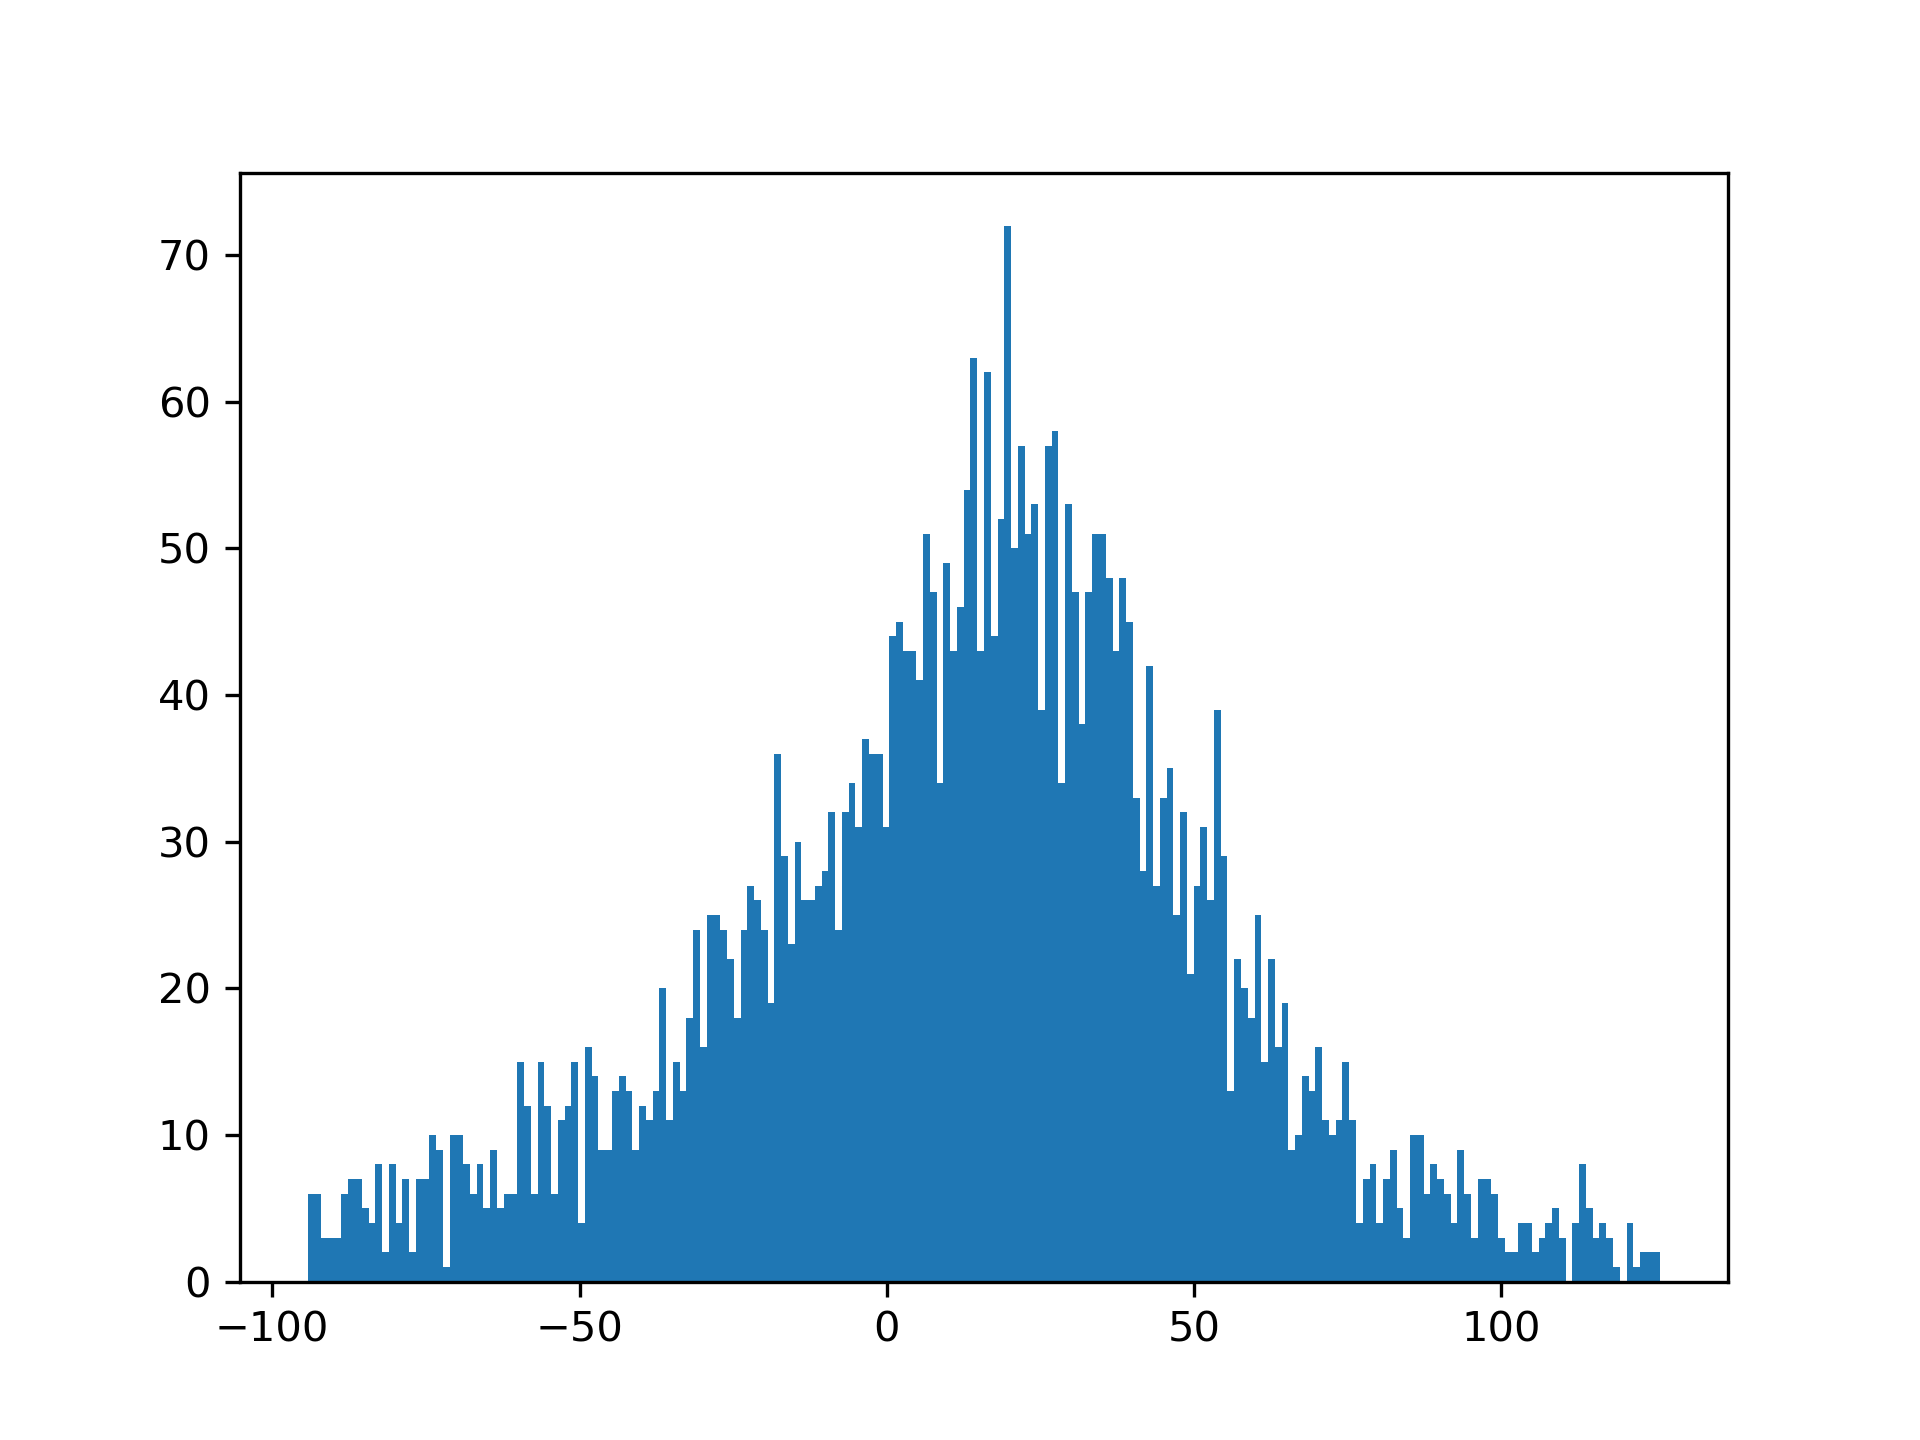
\includegraphics[width=\linewidth]{source/YHistogram.png}
    \caption{Histogram zmiennej objaśnianej}
\end{figure}

\newpage
\subsection{Korelacja}
Korelacja zmiennej objaśnianej ze zmiennymi objaśnianymi jest bardzo słaba, co wskazuje na potencjalnie silnie nieliniowy charakter zachodzących zależności.
\begin{table}[h!]
    \begin{center}
    \begin{tabular}{|c | c|} 
    \hline
    Statystyka & Wartość \\
    \hline\hline
    Średnia arytmetyczna & 0.0006535276131026212 \\ 
    \hline
    Odchylenie standardowe & 0.01430737685985159 \\
    \hline
    Kwartyl dolny & -0.006560508005214499 \\
    \hline
    Mediana & 0.0009029552423272379 \\
    \hline
    Kwartyl górny & 0.008516164727314403 \\
    \hline
    Wartość najmniejsza & -0.07707504123521973 \\
    \hline
    Wartość największa & 0.04058496958769639 \\
    \hline
    \end{tabular}
    \end{center}
   \caption{Korelacja zmiennej objaśnianej ze zmiennymi objaśnianymi}
\end{table}

\begin{figure}[h!]
    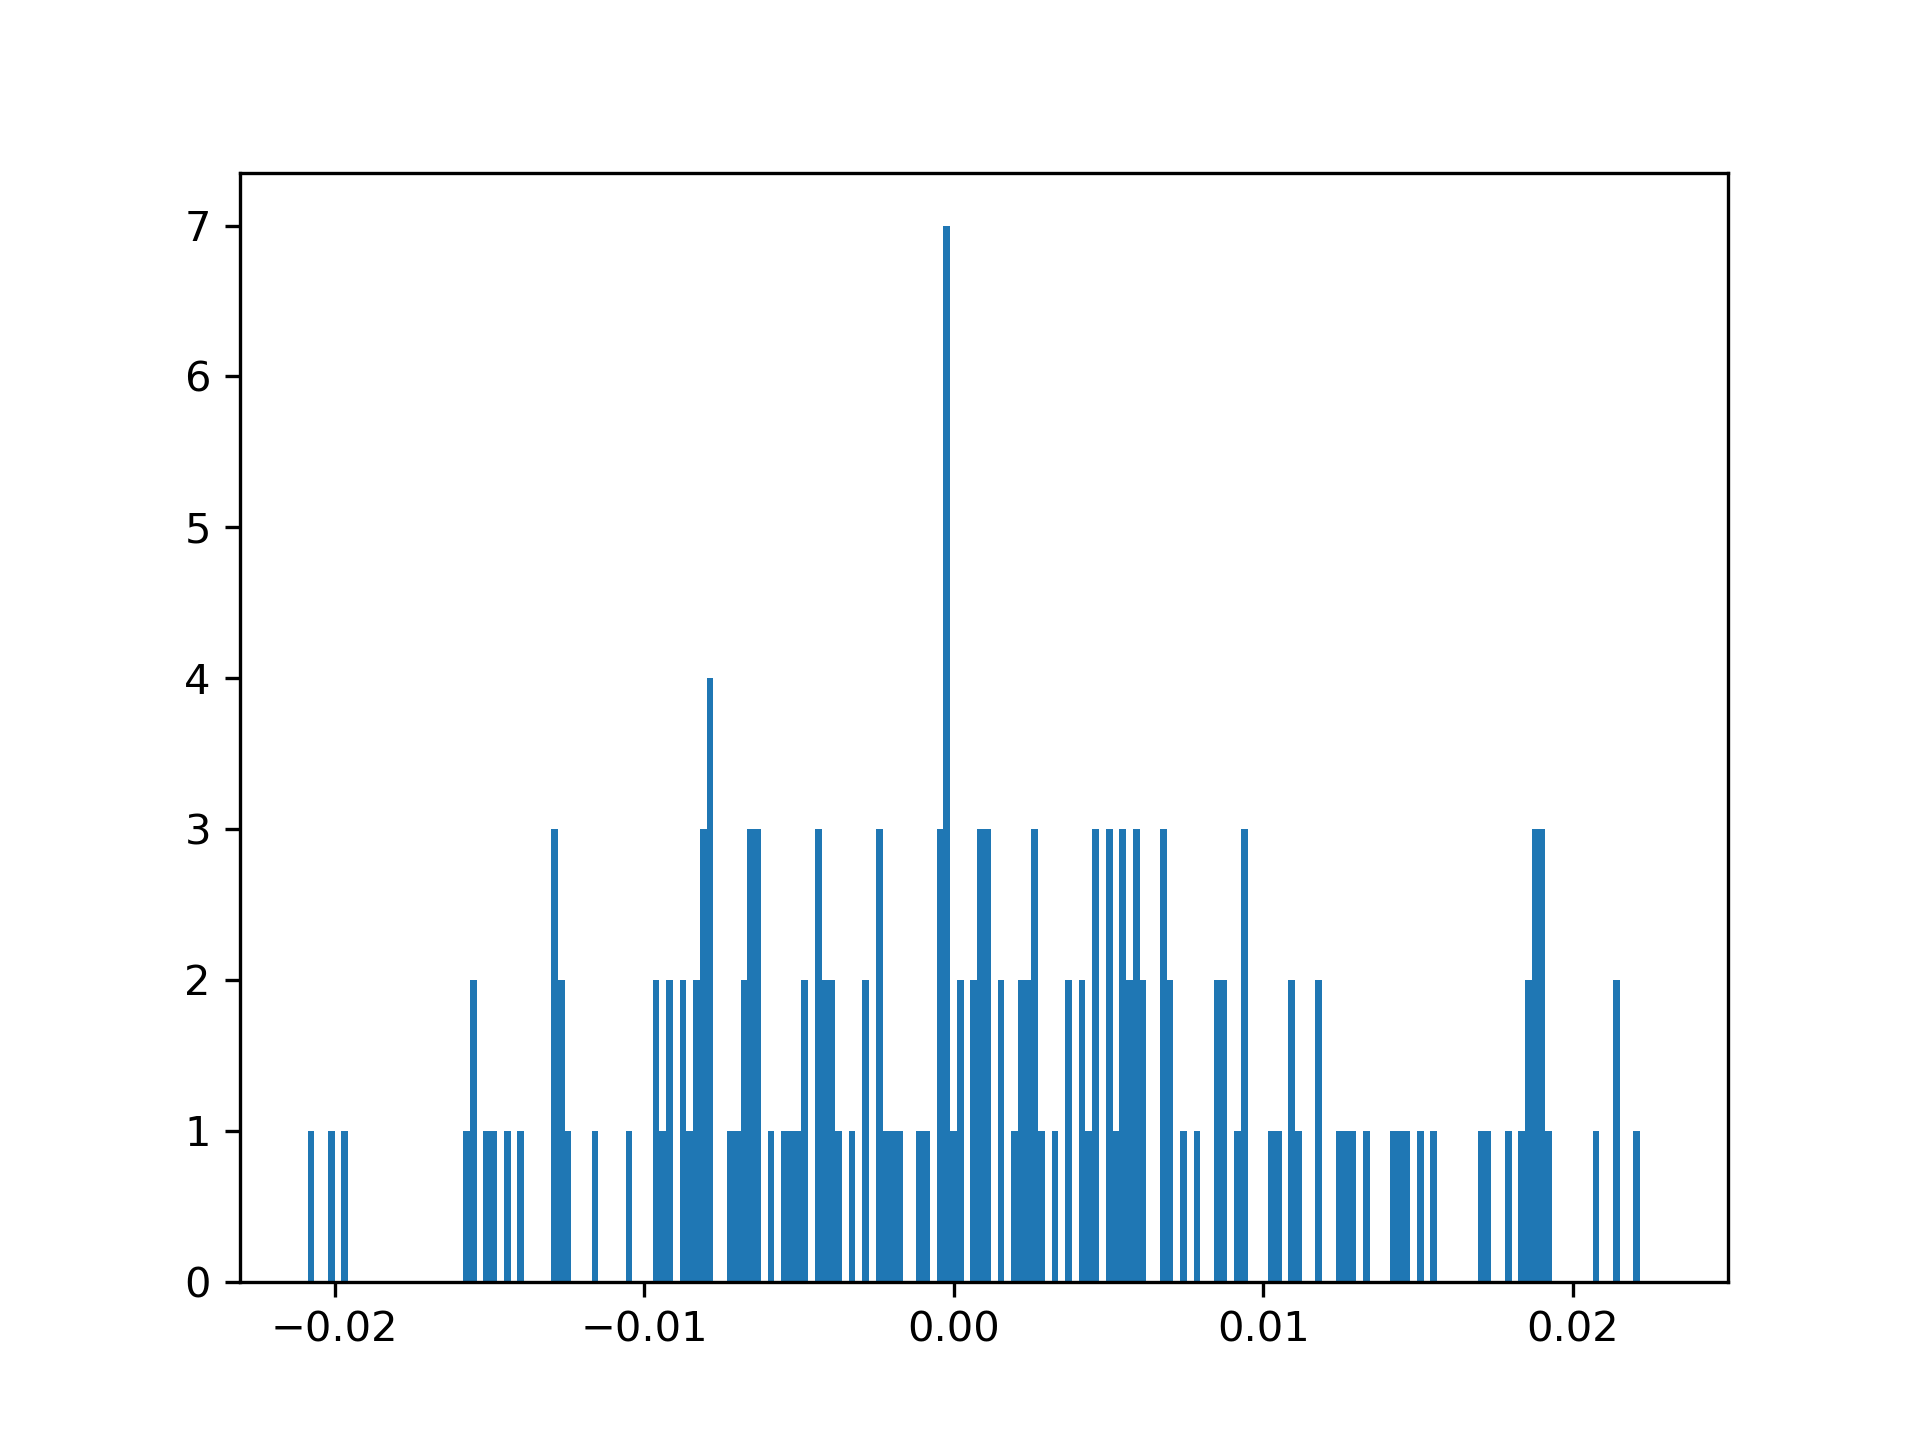
\includegraphics[width=\linewidth]{source/CorrHist.png}
    \caption{Histogram korelacji zmiennej objaśnianej ze zmiennymi objaśnianymi}
\end{figure}

\newpage
Korelacja pomiędzy niektórymi zmiennymi objaśniającymi jest silna, co można wyjaśnić zależnościami pomiędzy rozmiarem spółki, a wielkościami w \textit{10-K Form}. Nie wszystkie bazowe zmienne objaśniające mogą znaleźć się w modelu, ponieważ spowodowałoby to wystąpienie zjawiska współliniowości.
\begin{figure}[h!]
    \includegraphics[width=\linewidth]{source/CorrelationMatrix.png}
    \caption{Macierz korelacji}
\end{figure}

\subsection{Podział zbioru danych}
Zbiór danych podzielony jest na dane treningowe(90\%) użyte do estymacji parametrów modelów oraz dane testowe(10\%) służące do oceny prognozy \textit{ex post}.

\newpage
\section{Wybór postaci modelu oraz dobór zmiennych do modelu}
\subsection{Specyfikacja kryteriów}
Praca odpowiada na dwa pytania:
\begin{enumerate}
    \item Jaka jest bazowa efektywność predykcji?
    \item Jaki jest wpływ informacji zawartych w rozważanych danych na zmiany cen akcji?
\end{enumerate}

Odpowiedzią na pierwsze pytanie jest efektywność modelu o najlepszych właściwościach prognostycznych.

Odpowiedzią na drugie pytanie jest ocena współczynnika determinacji poprawnie zweryfikowanego modelu ekonometrycznego.

\subsection{Rozważana klasa funkcji}
Modele wybrane są z klasy funkcji dopuszczalnych ~$\mathscr{F}: \mathbb{R^K\to R}$,
gdzie K: liczba zmiennych w zbiorze danych.

Funkcje przyjmują analityczną postać:

~$\hat{Y}=a_0+a_1*X_1+...+a_k*X_k$;

parametry szacowane są przy użyciu metody najmniejszych kwadratów.

Ze względu na potencjalnie nielinowy charakter zależności rozważony został zbiór danych rozszerzony o przetransformowane zmienne: ~$e^{\frac{X_i-\overline{X_i}}{\sigma_{X_i}}}, X_i^2, X_i^3$ o łącznym rozmiarze 4392 x 748. Dalsze rozszerzanie zbioru danych osłabiło by stabilność numeryczną modeli i nadmiernie zwiększyło by wymiar Wapnika-Czerwonienkisa, co osłabiło by możliwości generalizacji przez modele (\textcite{Kaminski2017}).

\newpage
\subsection{Rozważany podzbiór funkcji}
Ze względu na ilość zmiennych, użycie metody o wykładniczej złożoności obliczeniowej, np. metody Hellwiga, byłoby nieefektywne. W związku z tym rozważany jest K-elementowy zbiór funkcji wyłoniony przy użyciu uproszczonej \textit{metody krokowej wstecz}. Rozważany jest model ze wszystkimi zmiennymi, a następnie z modelu usuwana jest najmniej istotna statystycznie zmienna. Procedura jest powtarzana dopóki w modelu jest więcej niż jedna zmienna. Dla celów stworzenia podzbioru funkcji nie jest sprawdzana normalność rozkładu resztowego.

\subsection{Kryterium wyboru modelu prognostycznego}
Spośród rozważanego podzbioru funkcji wybrana jest funkcja z najmniejszym \textit{absolutnym błędem prognozy ex post} oszacowanym przy użyciu sprawdzianu krzyżowego na danych treningowych.

Sprawdzian krzyżowy polega na podziale zboriu danych na J podzbiorów, a następnie wykonaniu J ocen błędu prognozy(za każdym razem inny podzbiór jest uznawany za testowy, J-1 podzbiorów treningowych) i obliczeniu ich średniej.

\[\hat{ME}= \frac{1}{J} \sum_{t=1}^{J} ( ME_i ) \]

\subsection{Kryterium wyboru modelu analitycznego}
Spośród rozważanego podzbioru funkcji wybrana jest funkcja z najwyższym współczynnikiem determinacji ~$R^2$, która została poprawnie zweryfikowana. W przypadku wystąpienia niepożadanych zjawisk w modelu, rozważany podzbiór funkcji powiększony zostaje o model z zastosowanymi stosownymi korektami.


\newpage
\section{Weryfikacja poprawności modelu}
Poniżej opisane są procedury weryfikacji poprawności modelu oszacowanego metodą najmniejszych kwadratów. Przyjęty poziom istotności ~$\alpha=0,05$.

\subsection{Współliniowość}
Wyznaczamy k modeli MNK, gdzie zmienną objaśnianą jest jedna ze zmiennych objaśniających, a zmiennymi objaśniającymi pozostałe zmienne. Wyznaczamy k współczynników determinacji; jeżeli którykolwiek z nich większy jest niż 0,9 , to w modelu występuje niepożądane zjawisko współiniowości zmiennych.

\subsection{Koincydencja}
Jeżeli dla każdego i=1..k:
\[sgn(r_i) = sgn(a_i)\],

gdzie:

~$r_i$: korelacja pomiędzy zmienną objaśnianą, a i-tą zmienną objaśniającą.

~$a_I$: oszacowany i-ty parametr modelu.

to model jest koincydentny. Koincydencja modelu jest pożądaną cechą.

\subsection{Efekt katalizy}
Niech ~$(X_i, X_j)$ będzie regularną parą korelacyjną. Wówczas jeżeli ~$r_{ij} < 0$ lub ~$r_{ij} > \frac{r_i}{r_j}$, gdzie:

~$r_{ij}$: korelacja między i-tą, a j-tą zmienną objaśniającą.

to zmienna ~$X_i$ jest katalizatorem. Poprawny model nie zawiera katalizatorów.

\newpage
\subsection{Normalność rozkładu reszt}
Normalność rozkładu składnika resztowego modelu jest cechą niezbędną do poprawnej interpretacji m.in. testów istotności parametrów modelu. Normalność rozkładu można zbadać przy użyciu testu Jarque-Bera.

~$H_0$: składnik losowy modelu ma rozkład normalny.

~$H_1$: składnik losowy modelu nie ma rozkładu normalnego.

Statystyka testowa ~$JB$ ma rozkład ~$\chi^2$ o dwóch stopniach swobody.

\[JB=\frac{n-k}{6}(A^2+\frac{1}{4}(K-3)^2)\],

gdzie:

Współczynnik skośności:
\[A = \frac{\hat{\mu}_3}{\hat{\sigma}^3} = 
\frac{\frac{1}{n} \sum_{t=1}^{n} ( x_t - \overline{x} )^3}
{(\frac{1}{n} \sum_{t=1}^{n} ( x_t - \overline{x} )^2)^{\frac{3}{2}}}
\]

Kurtoza:
\[K = \frac{\hat{\mu}_4}{\hat{\sigma}^4} = 
\frac{\frac{1}{n} \sum_{t=1}^{n} ( x_t - \overline{x} )^4}
{(\frac{1}{n} \sum_{t=1}^{n} ( x_t - \overline{x} )^2)^{2}}
\]

\subsection{Istotność zmiennych objaśniających}
Zmienne w poprawnym modelu są statystycznie istotne. Do badania istotności zmiennych służy test t-Studenta.

~$H_0$: ~$a_i = 0$.

~$H_1$: ~$a_i \neq 0$.

Statystyka testowa ~$t_{a_i}$ ma rozkład t-Studenta o n-(k+1) stopniach swobody.

\[t_{a_i} = \frac{a_i}{D(a_i)}\]

Dyspersja estymatora i-tego parametru modelu:

\[D(a_i)=\sqrt{d_{ii}}\]

Macierz kowariancji estymatora a:

\[\hat{D}^2(a)=S^2(X^TX)^{-1}\]

Estymator wariancji ~$s^2$ składnika losowego:

\[S^2 = \frac{e^Te}{n - (k + 1)}\]

\newpage
\subsection{Istotność współczynnika determinacji}
Istotność współczynnika determinacji(inaczej istotność wszystkich zmiennych naraz) jest pożądaną cechą modelu i może być zbadana za pomocą testu ~$F$.

~$H_0$: ~$a_1 = a_2 = ... = a_k = 0$.

~$H_1$: ~$a_1 \neq 0 \vee a_2 \neq 0 \vee ... \vee a_k \neq 0$.

Statystyka testowa ~$F$ ma rozkład F-Snedecora-Fishera z ~$r_1 = k$ i ~$r_2 = n - (k + 1)$ stopniami swobody.

\[F = \frac{R^2}{(1-R^2)}\frac{n - (k + 1)}{k}\]

\subsection{Liniowość postaci modelu}
Do badania liniowości modelu ekonometrycznego służy test serii.

~$H_0$: model hipotetyczny jest liniowy.

~$H_1$: model nie jest liniowy.

Statystyka testowa ~$Z$ ma asymptotyczny standardowy rozkład normalny.

~$r$ - liczba serii w wektorze resz modelu(uporządkowanych wg. wartości zmiennej objaśnianej).

~$N_1$ , ~$N_2$ - liczba dodatnich i ujemnych reszt modelu.

\[Z = \frac{r-(\frac{2N_1N_2}{n}+1)}{\sqrt{\frac{2N_1N_2(2N_1N_2-n)}{(n-1)n^2}}}\]

\subsection{Homoskedastyczność}
Homoskedastyczność jest pożądaną cechą modelu. Ze względu na wysoką proporcję ilości zmiennych objaśniających do ilości obserwacji homoskedastyczność najlepiej sprawdzić jest przy użyciu testu Goldfielda-Quandta.

~$H_0$: ~$s_1^2 = s_2^2$. Homoskedastyczność.

~$H_1$: ~$s_2^2 \neq s_2^2$. Heteroskedastyczność.

Statystyka testowa ~$F$ ma rozkład F-Snedecora-Fishera z ~$r_1 = n_1 - (k+1)$ i ~$r_2 = n_2 - (k + 1)$ stopniami swobody.

\[F = \frac{\hat{s}_1^2}{\hat{s}_2^2}\]

Próba podzielona jest na dwa zbiory i badana jest równość wariancji w podpróbach.

\[\hat{s}_1^2 = \frac{{e_1}^T{e_1}}{n_1-(k+1)}\]

\[\hat{s}_2^2 = \frac{{e_2}^T{e_2}}{n_2-(k+1)}\]

\newpage
\subsection{Stabilność parametrów modelu}
Stabilność parametrów modelu, która jest pożądana cechą, może zostać zweryfikowana przy pomocy testu Chowa.

~$H_0$: ~$\alpha = \beta = \gamma$. Paremetry modelu są stabilne.

~$H_1$: Parametry modelu nie są stabilne.

Statystyka testowa ~$F$ ma rozkład F-Snedecora-Fishera z ~$r_1 = k+1$ i ~$r_2 = n - 2(k + 1)$ stopniami swobody.

\[F = \frac{RSK - (RSK_1 + RSK_2)}{RSK_1 + RSK_2}\frac{n - 2(k+1)}{k + 1}\]

~$RSK$ - resztowa suma kwadratów oszacowanego modelu:

\[y_t = \alpha_0 + \alpha_1x_{1t}+...+\alpha_kx_{kt}+\epsilon_t,t=1,2,...,n\]

~$RSK_1$ - resztowa suma kwadratów oszacowanego modelu:

\[y_t = \beta_0 + \beta_1x_{1t}+...+\beta_kx_{kt}+\epsilon_{1t},t=1,2,...,n_1\]

~$RSK_2$ - resztowa suma kwadratów oszacowanego modelu:

\[y_t = \gamma_0 + \gamma_1x_{1t}+...+\gamma_kx_{kt}+\epsilon_{2t},t=n_1+1,n_1+2,...,n\]

\subsection{Autokorelacja składnika losowego}
Autokorelacja składnika losowego jest niepożądaną cechą modelu ekonometrycznego. Występowanie zjawiska autokorelacji pierwszego rzędu można badać przy założeniu, że:

\[e_t = \rho e_{t-1}+\eta_t\]

Służy do tego test mnożnika Lagrange'a autokorelacji składnika losowego.

~$H_0$: ~$\rho=0$. Zjawisko autokorelacji I rzędu nie występuje.

~$H_1$: ~$\rho\neq0$. Zjawisko autokorelacji I rzędu występuje.

Szacowany jest model pomocniczy i obliczany jest jego współczynnik determinacji.

\[e_t=\beta_0+\beta_1x_{1t}+\beta_2x_{2t}+...+\beta_kx_{kt}+\beta_{k+1}e_{t-1}+\mu_t\]

Dla dużej próby (~$n>30$) statystyka testowa ~$LM$ ma rozkład ~$\chi^2$ z jednym stopniem swobody.

\[LM = (n-1)R_{e_t}^2\]

\newpage
\section{Korekty}

\subsection{Korekty stabilności}
W związku z rozważaniem szerokiej klasy funkcji opartych o rozszerzony zbiór danych, a także dużą liczbę zmiennych objaśniających, korekty stabilności postaci modelu i stabilności parametrów nie są używane w projekcie.

\subsection{Korekta heteroskedastyczności i autokorelacji}

\subsubsection{Korekta heteroskedastyczności}
Do usunięcia heteroskedastyczności z modelu ekonometrycznego można użyć uogólnionej metody najmniejszych kwadratów.

Estymator parametrów modelu:

\[a = (X^T\Omega^{-1}X)^{-1}X^T\Omega^{-1}y\]

Estymator wariancji składnika losowego:

\[S^2=\frac{e^T\Omega^{-1}e}{n - (k+1)}\]

Estymator macierzy kowariancji estymatorów:

\[\hat{D}^2(a)=S^2(X^T\Omega^{-1}X)^{-1}\]

Macierz ~$\Omega$ nie jest znana, dlatego do korekt używa się estymatorów:

Korekta heteroskedastyczności dla ~$\sigma^2 = 1$ oraz estymatora ~$\sigma_t^2=e_t^2$:

\begin{equation*}
    \Omega_{h}^{-1}=
    \begin{bmatrix}
        \frac{1}{\sigma_1^2} & 0 & ... & 0 \\
        0 & \frac{1}{\sigma_2^2} & ... & 0 \\
        ... & ... & ... & ... \\
        0 & 0 & ... & \frac{1}{\sigma_n^2}
    \end{bmatrix}
\end{equation*}

Zatem korekta odpowiada transformacji zmiennych:

\[Y_t^* = \frac{Y_t}{\sqrt{e_t^2}}\]

\[X_{it}^* = \frac{X_{it}}{\sqrt{e_t^2}}\]

\newpage
\subsubsection{Korekta autokorelacji I rzędu}
Korekta autokorelacji I rzędu przy użyciu metody Cochrane'a-Orcutta:

\[Y_t^* = Y_t - \hat{\rho}Y_{t-1}\]

\[X_{it}^* = X_{it} - \hat{\rho}X_{it-1}\]

\[Y_1^* = Y_1\sqrt{1-\hat{\rho}^2}\]

\[X_{i1}^* = X_{i1}\sqrt{1 - \hat{\rho}^2}\]

\subsubsection{Korekta łączna}
Korektę łączną zapisać można jako(~$\rho$ wyestymowane po korekcie heteroskedastyczności):

\[Y_t^* = \frac{Y_t}{\sqrt{e_t^2}} - \hat{\rho}\frac{Y_{t-1}}{\sqrt{e_{t-1}^2}}\]

\[Y_1^* = \frac{Y_1}{\sqrt{e_1^2}}\sqrt{1-\hat{\rho}^2}\]

\[X_{it}^* = \frac{X_{it}}{\sqrt{e_t^2}} - \hat{\rho}\frac{X_{it-1}}{\sqrt{e_{t-1}^2}}\]

\[X_{i1}^* = \frac{X_{i1}}{\sqrt{e_1^2}}\sqrt{1-\hat{\rho}}\]

\newpage
\section{Wybrane modele}
\subsection{Wybór modelu}
Dla celów wyboru modelu klasa funkcji została rozszerzona o modele z korektą heteroskedastyczności, korektą autokorelacji oraz korektą łączną, co zwiększyło ilość rozważanych modeli do ~$4K=4*748=2992$. Poprawność każdego rozważanego modelu została zweryfikowana. Pełne sprawozdanie z estymacji i weryfikacji wszystkich modeli znajduje się w załączniku do pracy.

\subsection{Model prognostyczny}
\subsubsection{Postać modelu}
\[ \hat{Y} = \alpha_0\]
\[+\alpha_{1}EPS Diluted\]
\[+\alpha_{2}netProfitMargin\]
\[+\alpha_{3}returnOnEquity\]
\[+\alpha_{4}daysOfSalesOutstanding\]
\[+\alpha_{5}PE ratio\]
\[+\alpha_{6}POCF ratio\]
\[+\alpha_{7}Operating Income Growth\]
\[+\alpha_{8}Asset Growth\]
\[+\alpha_{9}Technology\]
\[+\alpha_{10}Utilities\]
\[+\alpha_{11}e^{\frac{Cost of Revenue - \overline{Cost of Revenue}}{\sigma_{Cost of Revenue}}}\]
\[+\alpha_{12}Net Income - Non-Controlling int^2\]
\[+\alpha_{13}Net Income^2\]
\[+\alpha_{14}Preferred Dividends^2\]
\[+\alpha_{15}Net Income Com^3\]
\[+\alpha_{16}e^{\frac{EPS - \overline{EPS}}{\sigma_{EPS}}}\]
\[+\alpha_{17}EPS^2\]
\[+\alpha_{18}EBITDA Margin^3\]
\[+\alpha_{19}EBIT^3\]
\[+\alpha_{20}e^{\frac{Earnings Before Tax Margin - \overline{Earnings Before Tax Margin}}{\sigma_{Earnings Before Tax Margin}}}\]
\[+\alpha_{21}Cash and short-term investments^2\]
\[+\alpha_{22}Goodwill and Intangible Assets^2\]
\[+\alpha_{23}Goodwill and Intangible Assets^3\]
\[+\alpha_{24}e^{\frac{Total assets - \overline{Total assets}}{\sigma_{Total assets}}}\]
\[+\alpha_{25}Total assets^2\]
\[+\alpha_{26}e^{\frac{Total debt - \overline{Total debt}}{\sigma_{Total debt}}}\]
\[+\alpha_{27}Other comprehensive income^3\]
\[+\alpha_{28}Retained earnings (deficit)^2\]
\[+\alpha_{29}Net Debt^2\]
\[+\alpha_{30}e^{\frac{Operating Cash Flow - \overline{Operating Cash Flow}}{\sigma_{Operating Cash Flow}}}\]
\[+\alpha_{31}Capital Expenditure^3\]
\[+\alpha_{32}e^{\frac{Acquisitions and disposals - \overline{Acquisitions and disposals}}{\sigma_{Acquisitions and disposals}}}\]
\[+\alpha_{33}e^{\frac{Issuance (repayment) of debt - \overline{Issuance (repayment) of debt}}{\sigma_{Issuance (repayment) of debt}}}\]
\[+\alpha_{34}Financing Cash Flow^2\]
\[+\alpha_{35}priceSalesRatio^3\]
\[+\alpha_{36}pretaxProfitMargin^3\]
\[+\alpha_{37}interestCoverage^3\]
\[+\alpha_{38}e^{\frac{companyEquityMultiplier - \overline{companyEquityMultiplier}}{\sigma_{companyEquityMultiplier}}}\]
\[+\alpha_{39}companyEquityMultiplier^3\]
\[+\alpha_{40}operatingCashFlowPerShare^3\]
\[+\alpha_{41}e^{\frac{capitalExpenditureCoverageRatios - \overline{capitalExpenditureCoverageRatios}}{\sigma_{capitalExpenditureCoverageRatios}}}\]
\[+\alpha_{42}Debt to Equity^2\]
\[+\alpha_{43}e^{\frac{Income Quality - \overline{Income Quality}}{\sigma_{Income Quality}}}\]
\[+\alpha_{44}e^{\frac{SGAndA to Revenue - \overline{SGAndA to Revenue}}{\sigma_{SGAndA to Revenue}}}\]
\[+\alpha_{45}e^{\frac{RAndD to Revenue - \overline{RAndD to Revenue}}{\sigma_{RAndD to Revenue}}}\]
\[+\alpha_{46}Capex to Depreciation^3\]
\[+\alpha_{47}Stock-based compensation to Revenue^2\]
\[+\alpha_{48}e^{\frac{Net Current Asset Value - \overline{Net Current Asset Value}}{\sigma_{Net Current Asset Value}}}\]
\[+\alpha_{49}Net Current Asset Value^2\]
\[+\alpha_{50}Net Current Asset Value^3\]
\[+\alpha_{51}e^{\frac{Average Payables - \overline{Average Payables}}{\sigma_{Average Payables}}}\]
\[+\alpha_{52}Days of Inventory on Hand^2\]
\[+\alpha_{53}Days of Inventory on Hand^3\]
\[+\alpha_{54}Payables Turnover^2\]
\[+\alpha_{55}EPS Growth^2\]
\[+\alpha_{56}EPS Growth^3\]
\[+\alpha_{57}Operating Cash Flow growth^3\]
\[+\alpha_{58}3Y Net Income Growth (per Share)^3\]
\[+\alpha_{59}e^{\frac{SGAndA Expenses Growth - \overline{SGAndA Expenses Growth}}{\sigma_{SGAndA Expenses Growth}}}\]
\[+\alpha_{60}e^{\frac{Consumer Defensive - \overline{Consumer Defensive}}{\sigma_{Consumer Defensive}}}\]
\[+\alpha_{61}e^{\frac{Utilities - \overline{Utilities}}{\sigma_{Utilities}}}\]
\subsubsection{Wyestymowane parametry modelu}
\[\alpha_{0} = 2018.5477815770553\]
\[\alpha_{1} = 0.03291365678978788\]
\[\alpha_{2} = 0.00020374174789324775\]
\[\alpha_{3} = -0.004858593987936153\]
\[\alpha_{4} = 0.005942199011346903\]
\[\alpha_{5} = 0.019366139832899386\]
\[\alpha_{6} = -0.005747608907094429\]
\[\alpha_{7} = -0.005572801679067712\]
\[\alpha_{8} = 0.007614463032898771\]
\[\alpha_{9} = 5.276455632720324\]
\[\alpha_{10} = 1337633.129234511\]
\[\alpha_{11} = -9.11510095048615e-11\]
\[\alpha_{12} = 1.985032302628627e-18\]
\[\alpha_{13} = 6.594869219173502e-20\]
\[\alpha_{14} = -6.523048257641268e-18\]
\[\alpha_{15} = -1.0319980322228234e-30\]
\[\alpha_{16} = -0.00011515820201976649\]
\[\alpha_{17} = 7.806455171671651e-08\]
\[\alpha_{18} = -1.3215034600680261e-11\]
\[\alpha_{19} = 1.4264304686694543e-31\]
\[\alpha_{20} = 0.012680635305010669\]
\[\alpha_{21} = 8.382352042166059e-23\]
\[\alpha_{22} = -3.1471143144034345e-23\]
\[\alpha_{23} = 1.4340162420583117e-33\]
\[\alpha_{24} = -2.5427122707594187e-08\]
\[\alpha_{25} = -1.109847115918334e-23\]
\[\alpha_{26} = 2.7732381814810168e-08\]
\[\alpha_{27} = 3.698001298539986e-33\]
\[\alpha_{28} = -1.7983616168878857e-22\]
\[\alpha_{29} = 4.09817668810202e-24\]
\[\alpha_{30} = -2.3559504394199613e-10\]
\[\alpha_{31} = 1.9602927836776526e-30\]
\[\alpha_{32} = -0.028497353021586666\]
\[\alpha_{33} = -1.4990159003832128e-08\]
\[\alpha_{34} = -3.5109674794177256e-22\]
\[\alpha_{35} = -8.002350777799246e-12\]
\[\alpha_{36} = -1.0419376515929007e-08\]
\[\alpha_{37} = 1.888116317683361e-14\]
\[\alpha_{38} = -5.886733199583766e-20\]
\[\alpha_{39} = 6.62321625182638e-13\]
\[\alpha_{40} = -1.3076861165287683e-22\]
\[\alpha_{41} = 0.35971539702278993\]
\[\alpha_{42} = -0.00019950883606210482\]
\[\alpha_{43} = -1.0791618948143402e-10\]
\[\alpha_{44} = 4.046652112303246e-14\]
\[\alpha_{45} = -4.378960854447986e-12\]
\[\alpha_{46} = 1.3735877552681745e-07\]
\[\alpha_{47} = 0.0002618314457154143\]
\[\alpha_{48} = -4.123736451202189\]
\[\alpha_{49} = -2.8515037106406942e-24\]
\[\alpha_{50} = -1.6804667725574223e-35\]
\[\alpha_{51} = 1.2229626226962909e-21\]
\[\alpha_{52} = 2.3530287024025934e-07\]
\[\alpha_{53} = 4.517875758929235e-14\]
\[\alpha_{54} = -1.206295182175142e-06\]
\[\alpha_{55} = 0.0004976025581231616\]
\[\alpha_{56} = -3.6618986315734903e-06\]
\[\alpha_{57} = 3.495342885919652e-10\]
\[\alpha_{58} = -0.020813179975838824\]
\[\alpha_{59} = -8.300856564349884e-22\]
\[\alpha_{60} = 0.04315768012612904\]
\[\alpha_{61} = -2284.6940223375314\]
\subsubsection{Wskaźniki jakości modelu}
Współczynnik determinacji ~$R^2 = 0.8572313515395971$

Średni absolutny błąd prognozy \textit{ex post} ~$MAE = 40.320489091071536$

\subsubsection{Weryfikacja poprawności modelu}
Weryfikacja poprawności modelu przy poziomie istotności ~$\alpha = 0.05$
\subsubsection{Koincydencja}
\[sgn(\alpha_{1}) = 1\]
\[sgn(r_{1}) = 1\]
Koincydencja.
\[sgn(\alpha_{2}) = 1\]
\[sgn(r_{2}) = -1\]
Brak koincydencji.
\[sgn(\alpha_{3}) = -1\]
\[sgn(r_{3}) = -1\]
Koincydencja.
\[sgn(\alpha_{4}) = 1\]
\[sgn(r_{4}) = -1\]
Brak koincydencji.
\[sgn(\alpha_{5}) = 1\]
\[sgn(r_{5}) = 1\]
Koincydencja.
\[sgn(\alpha_{6}) = -1\]
\[sgn(r_{6}) = -1\]
Koincydencja.
\[sgn(\alpha_{7}) = -1\]
\[sgn(r_{7}) = 1\]
Brak koincydencji.
\[sgn(\alpha_{8}) = 1\]
\[sgn(r_{8}) = -1\]
Brak koincydencji.
\[sgn(\alpha_{9}) = 1\]
\[sgn(r_{9}) = 1\]
Koincydencja.
\[sgn(\alpha_{10}) = 1\]
\[sgn(r_{10}) = 1\]
Koincydencja.
\[sgn(\alpha_{11}) = -1\]
\[sgn(r_{11}) = 1\]
Brak koincydencji.
\[sgn(\alpha_{12}) = 1\]
\[sgn(r_{12}) = -1\]
Brak koincydencji.
\[sgn(\alpha_{13}) = 1\]
\[sgn(r_{13}) = 1\]
Koincydencja.
\[sgn(\alpha_{14}) = -1\]
\[sgn(r_{14}) = 1\]
Brak koincydencji.
\[sgn(\alpha_{15}) = -1\]
\[sgn(r_{15}) = 1\]
Brak koincydencji.
\[sgn(\alpha_{16}) = -1\]
\[sgn(r_{16}) = 1\]
Brak koincydencji.
\[sgn(\alpha_{17}) = 1\]
\[sgn(r_{17}) = -1\]
Brak koincydencji.
\[sgn(\alpha_{18}) = -1\]
\[sgn(r_{18}) = -1\]
Koincydencja.
\[sgn(\alpha_{19}) = 1\]
\[sgn(r_{19}) = 1\]
Koincydencja.
\[sgn(\alpha_{20}) = 1\]
\[sgn(r_{20}) = 1\]
Koincydencja.
\[sgn(\alpha_{21}) = 1\]
\[sgn(r_{21}) = 1\]
Koincydencja.
\[sgn(\alpha_{22}) = -1\]
\[sgn(r_{22}) = 1\]
Brak koincydencji.
\[sgn(\alpha_{23}) = 1\]
\[sgn(r_{23}) = 1\]
Koincydencja.
\[sgn(\alpha_{24}) = -1\]
\[sgn(r_{24}) = 1\]
Brak koincydencji.
\[sgn(\alpha_{25}) = -1\]
\[sgn(r_{25}) = 1\]
Brak koincydencji.
\[sgn(\alpha_{26}) = 1\]
\[sgn(r_{26}) = 1\]
Koincydencja.
\[sgn(\alpha_{27}) = 1\]
\[sgn(r_{27}) = 1\]
Koincydencja.
\[sgn(\alpha_{28}) = -1\]
\[sgn(r_{28}) = -1\]
Koincydencja.
\[sgn(\alpha_{29}) = 1\]
\[sgn(r_{29}) = 1\]
Koincydencja.
\[sgn(\alpha_{30}) = -1\]
\[sgn(r_{30}) = -1\]
Koincydencja.
\[sgn(\alpha_{31}) = 1\]
\[sgn(r_{31}) = 1\]
Koincydencja.
\[sgn(\alpha_{32}) = -1\]
\[sgn(r_{32}) = 1\]
Brak koincydencji.
\[sgn(\alpha_{33}) = -1\]
\[sgn(r_{33}) = 1\]
Brak koincydencji.
\[sgn(\alpha_{34}) = -1\]
\[sgn(r_{34}) = -1\]
Koincydencja.
\[sgn(\alpha_{35}) = -1\]
\[sgn(r_{35}) = -1\]
Koincydencja.
\[sgn(\alpha_{36}) = -1\]
\[sgn(r_{36}) = -1\]
Koincydencja.
\[sgn(\alpha_{37}) = 1\]
\[sgn(r_{37}) = 1\]
Koincydencja.
\[sgn(\alpha_{38}) = -1\]
\[sgn(r_{38}) = -1\]
Koincydencja.
\[sgn(\alpha_{39}) = 1\]
\[sgn(r_{39}) = -1\]
Brak koincydencji.
\[sgn(\alpha_{40}) = -1\]
\[sgn(r_{40}) = -1\]
Koincydencja.
\[sgn(\alpha_{41}) = 1\]
\[sgn(r_{41}) = -1\]
Brak koincydencji.
\[sgn(\alpha_{42}) = -1\]
\[sgn(r_{42}) = -1\]
Koincydencja.
\[sgn(\alpha_{43}) = -1\]
\[sgn(r_{43}) = -1\]
Koincydencja.
\[sgn(\alpha_{44}) = 1\]
\[sgn(r_{44}) = -1\]
Brak koincydencji.
\[sgn(\alpha_{45}) = -1\]
\[sgn(r_{45}) = -1\]
Koincydencja.
\[sgn(\alpha_{46}) = 1\]
\[sgn(r_{46}) = 1\]
Koincydencja.
\[sgn(\alpha_{47}) = 1\]
\[sgn(r_{47}) = 1\]
Koincydencja.
\[sgn(\alpha_{48}) = -1\]
\[sgn(r_{48}) = -1\]
Koincydencja.
\[sgn(\alpha_{49}) = -1\]
\[sgn(r_{49}) = 1\]
Brak koincydencji.
\[sgn(\alpha_{50}) = -1\]
\[sgn(r_{50}) = -1\]
Koincydencja.
\[sgn(\alpha_{51}) = 1\]
\[sgn(r_{51}) = -1\]
Brak koincydencji.
\[sgn(\alpha_{52}) = 1\]
\[sgn(r_{52}) = 1\]
Koincydencja.
\[sgn(\alpha_{53}) = 1\]
\[sgn(r_{53}) = -1\]
Brak koincydencji.
\[sgn(\alpha_{54}) = -1\]
\[sgn(r_{54}) = -1\]
Koincydencja.
\[sgn(\alpha_{55}) = 1\]
\[sgn(r_{55}) = -1\]
Brak koincydencji.
\[sgn(\alpha_{56}) = -1\]
\[sgn(r_{56}) = -1\]
Koincydencja.
\[sgn(\alpha_{57}) = 1\]
\[sgn(r_{57}) = 1\]
Koincydencja.
\[sgn(\alpha_{58}) = -1\]
\[sgn(r_{58}) = -1\]
Koincydencja.
\[sgn(\alpha_{59}) = -1\]
\[sgn(r_{59}) = -1\]
Koincydencja.
\[sgn(\alpha_{60}) = 1\]
\[sgn(r_{60}) = 1\]
Koincydencja.
\[sgn(\alpha_{61}) = -1\]
\[sgn(r_{61}) = 1\]
Brak koincydencji.
\subsubsection{Katalizatory}
Zmienna ~$X_{2}$ jest katalizatorem w parze (~$X_{2}$, ~$X_{1}$)

Zmienna ~$X_{2}$ jest katalizatorem w parze (~$X_{2}$, ~$X_{5}$)

Zmienna ~$X_{2}$ jest katalizatorem w parze (~$X_{2}$, ~$X_{9}$)

Zmienna ~$X_{2}$ jest katalizatorem w parze (~$X_{2}$, ~$X_{20}$)

Zmienna ~$X_{2}$ jest katalizatorem w parze (~$X_{2}$, ~$X_{47}$)

Zmienna ~$X_{3}$ jest katalizatorem w parze (~$X_{3}$, ~$X_{1}$)

Zmienna ~$X_{3}$ jest katalizatorem w parze (~$X_{3}$, ~$X_{6}$)

Zmienna ~$X_{3}$ jest katalizatorem w parze (~$X_{3}$, ~$X_{8}$)

Zmienna ~$X_{3}$ jest katalizatorem w parze (~$X_{3}$, ~$X_{12}$)

Zmienna ~$X_{3}$ jest katalizatorem w parze (~$X_{3}$, ~$X_{17}$)

Zmienna ~$X_{3}$ jest katalizatorem w parze (~$X_{3}$, ~$X_{31}$)

Zmienna ~$X_{3}$ jest katalizatorem w parze (~$X_{3}$, ~$X_{35}$)

Zmienna ~$X_{3}$ jest katalizatorem w parze (~$X_{3}$, ~$X_{37}$)

Zmienna ~$X_{3}$ jest katalizatorem w parze (~$X_{3}$, ~$X_{40}$)

Zmienna ~$X_{3}$ jest katalizatorem w parze (~$X_{3}$, ~$X_{41}$)

Zmienna ~$X_{3}$ jest katalizatorem w parze (~$X_{3}$, ~$X_{42}$)

Zmienna ~$X_{3}$ jest katalizatorem w parze (~$X_{3}$, ~$X_{43}$)

Zmienna ~$X_{3}$ jest katalizatorem w parze (~$X_{3}$, ~$X_{44}$)

Zmienna ~$X_{3}$ jest katalizatorem w parze (~$X_{3}$, ~$X_{45}$)

Zmienna ~$X_{3}$ jest katalizatorem w parze (~$X_{3}$, ~$X_{46}$)

Zmienna ~$X_{3}$ jest katalizatorem w parze (~$X_{3}$, ~$X_{51}$)

Zmienna ~$X_{3}$ jest katalizatorem w parze (~$X_{3}$, ~$X_{54}$)

Zmienna ~$X_{3}$ jest katalizatorem w parze (~$X_{3}$, ~$X_{57}$)

Zmienna ~$X_{3}$ jest katalizatorem w parze (~$X_{3}$, ~$X_{58}$)

Zmienna ~$X_{3}$ jest katalizatorem w parze (~$X_{3}$, ~$X_{59}$)

Zmienna ~$X_{4}$ jest katalizatorem w parze (~$X_{4}$, ~$X_{2}$)

Zmienna ~$X_{4}$ jest katalizatorem w parze (~$X_{4}$, ~$X_{5}$)

Zmienna ~$X_{4}$ jest katalizatorem w parze (~$X_{4}$, ~$X_{9}$)

Zmienna ~$X_{4}$ jest katalizatorem w parze (~$X_{4}$, ~$X_{10}$)

Zmienna ~$X_{4}$ jest katalizatorem w parze (~$X_{4}$, ~$X_{13}$)

Zmienna ~$X_{4}$ jest katalizatorem w parze (~$X_{4}$, ~$X_{15}$)

Zmienna ~$X_{4}$ jest katalizatorem w parze (~$X_{4}$, ~$X_{16}$)

Zmienna ~$X_{4}$ jest katalizatorem w parze (~$X_{4}$, ~$X_{19}$)

Zmienna ~$X_{4}$ jest katalizatorem w parze (~$X_{4}$, ~$X_{20}$)

Zmienna ~$X_{4}$ jest katalizatorem w parze (~$X_{4}$, ~$X_{47}$)

Zmienna ~$X_{4}$ jest katalizatorem w parze (~$X_{4}$, ~$X_{52}$)

Zmienna ~$X_{4}$ jest katalizatorem w parze (~$X_{4}$, ~$X_{53}$)

Zmienna ~$X_{4}$ jest katalizatorem w parze (~$X_{4}$, ~$X_{61}$)

Zmienna ~$X_{6}$ jest katalizatorem w parze (~$X_{6}$, ~$X_{9}$)

Zmienna ~$X_{6}$ jest katalizatorem w parze (~$X_{6}$, ~$X_{17}$)

Zmienna ~$X_{6}$ jest katalizatorem w parze (~$X_{6}$, ~$X_{54}$)

Zmienna ~$X_{7}$ jest katalizatorem w parze (~$X_{7}$, ~$X_{2}$)

Zmienna ~$X_{7}$ jest katalizatorem w parze (~$X_{7}$, ~$X_{3}$)

Zmienna ~$X_{7}$ jest katalizatorem w parze (~$X_{7}$, ~$X_{4}$)

Zmienna ~$X_{7}$ jest katalizatorem w parze (~$X_{7}$, ~$X_{9}$)

Zmienna ~$X_{7}$ jest katalizatorem w parze (~$X_{7}$, ~$X_{10}$)

Zmienna ~$X_{7}$ jest katalizatorem w parze (~$X_{7}$, ~$X_{11}$)

Zmienna ~$X_{7}$ jest katalizatorem w parze (~$X_{7}$, ~$X_{13}$)

Zmienna ~$X_{7}$ jest katalizatorem w parze (~$X_{7}$, ~$X_{14}$)

Zmienna ~$X_{7}$ jest katalizatorem w parze (~$X_{7}$, ~$X_{15}$)

Zmienna ~$X_{7}$ jest katalizatorem w parze (~$X_{7}$, ~$X_{17}$)

Zmienna ~$X_{7}$ jest katalizatorem w parze (~$X_{7}$, ~$X_{18}$)

Zmienna ~$X_{7}$ jest katalizatorem w parze (~$X_{7}$, ~$X_{19}$)

Zmienna ~$X_{7}$ jest katalizatorem w parze (~$X_{7}$, ~$X_{20}$)

Zmienna ~$X_{7}$ jest katalizatorem w parze (~$X_{7}$, ~$X_{21}$)

Zmienna ~$X_{7}$ jest katalizatorem w parze (~$X_{7}$, ~$X_{22}$)

Zmienna ~$X_{7}$ jest katalizatorem w parze (~$X_{7}$, ~$X_{23}$)

Zmienna ~$X_{7}$ jest katalizatorem w parze (~$X_{7}$, ~$X_{24}$)

Zmienna ~$X_{7}$ jest katalizatorem w parze (~$X_{7}$, ~$X_{25}$)

Zmienna ~$X_{7}$ jest katalizatorem w parze (~$X_{7}$, ~$X_{26}$)

Zmienna ~$X_{7}$ jest katalizatorem w parze (~$X_{7}$, ~$X_{29}$)

Zmienna ~$X_{7}$ jest katalizatorem w parze (~$X_{7}$, ~$X_{32}$)

Zmienna ~$X_{7}$ jest katalizatorem w parze (~$X_{7}$, ~$X_{33}$)

Zmienna ~$X_{7}$ jest katalizatorem w parze (~$X_{7}$, ~$X_{38}$)

Zmienna ~$X_{7}$ jest katalizatorem w parze (~$X_{7}$, ~$X_{39}$)

Zmienna ~$X_{7}$ jest katalizatorem w parze (~$X_{7}$, ~$X_{42}$)

Zmienna ~$X_{7}$ jest katalizatorem w parze (~$X_{7}$, ~$X_{43}$)

Zmienna ~$X_{7}$ jest katalizatorem w parze (~$X_{7}$, ~$X_{47}$)

Zmienna ~$X_{7}$ jest katalizatorem w parze (~$X_{7}$, ~$X_{48}$)

Zmienna ~$X_{7}$ jest katalizatorem w parze (~$X_{7}$, ~$X_{49}$)

Zmienna ~$X_{7}$ jest katalizatorem w parze (~$X_{7}$, ~$X_{50}$)

Zmienna ~$X_{7}$ jest katalizatorem w parze (~$X_{7}$, ~$X_{52}$)

Zmienna ~$X_{7}$ jest katalizatorem w parze (~$X_{7}$, ~$X_{53}$)

Zmienna ~$X_{7}$ jest katalizatorem w parze (~$X_{7}$, ~$X_{54}$)

Zmienna ~$X_{7}$ jest katalizatorem w parze (~$X_{7}$, ~$X_{56}$)

Zmienna ~$X_{7}$ jest katalizatorem w parze (~$X_{7}$, ~$X_{58}$)

Zmienna ~$X_{7}$ jest katalizatorem w parze (~$X_{7}$, ~$X_{59}$)

Zmienna ~$X_{7}$ jest katalizatorem w parze (~$X_{7}$, ~$X_{61}$)

Zmienna ~$X_{8}$ jest katalizatorem w parze (~$X_{8}$, ~$X_{1}$)

Zmienna ~$X_{8}$ jest katalizatorem w parze (~$X_{8}$, ~$X_{2}$)

Zmienna ~$X_{8}$ jest katalizatorem w parze (~$X_{8}$, ~$X_{4}$)

Zmienna ~$X_{8}$ jest katalizatorem w parze (~$X_{8}$, ~$X_{5}$)

Zmienna ~$X_{8}$ jest katalizatorem w parze (~$X_{8}$, ~$X_{6}$)

Zmienna ~$X_{8}$ jest katalizatorem w parze (~$X_{8}$, ~$X_{17}$)

Zmienna ~$X_{8}$ jest katalizatorem w parze (~$X_{8}$, ~$X_{31}$)

Zmienna ~$X_{8}$ jest katalizatorem w parze (~$X_{8}$, ~$X_{37}$)

Zmienna ~$X_{8}$ jest katalizatorem w parze (~$X_{8}$, ~$X_{40}$)

Zmienna ~$X_{8}$ jest katalizatorem w parze (~$X_{8}$, ~$X_{41}$)

Zmienna ~$X_{8}$ jest katalizatorem w parze (~$X_{8}$, ~$X_{42}$)

Zmienna ~$X_{8}$ jest katalizatorem w parze (~$X_{8}$, ~$X_{43}$)

Zmienna ~$X_{8}$ jest katalizatorem w parze (~$X_{8}$, ~$X_{46}$)

Zmienna ~$X_{8}$ jest katalizatorem w parze (~$X_{8}$, ~$X_{52}$)

Zmienna ~$X_{8}$ jest katalizatorem w parze (~$X_{8}$, ~$X_{53}$)

Zmienna ~$X_{8}$ jest katalizatorem w parze (~$X_{8}$, ~$X_{54}$)

Zmienna ~$X_{8}$ jest katalizatorem w parze (~$X_{8}$, ~$X_{58}$)

Zmienna ~$X_{10}$ jest katalizatorem w parze (~$X_{10}$, ~$X_{2}$)

Zmienna ~$X_{10}$ jest katalizatorem w parze (~$X_{10}$, ~$X_{9}$)

Zmienna ~$X_{10}$ jest katalizatorem w parze (~$X_{10}$, ~$X_{13}$)

Zmienna ~$X_{10}$ jest katalizatorem w parze (~$X_{10}$, ~$X_{15}$)

Zmienna ~$X_{10}$ jest katalizatorem w parze (~$X_{10}$, ~$X_{16}$)

Zmienna ~$X_{10}$ jest katalizatorem w parze (~$X_{10}$, ~$X_{19}$)

Zmienna ~$X_{10}$ jest katalizatorem w parze (~$X_{10}$, ~$X_{20}$)

Zmienna ~$X_{10}$ jest katalizatorem w parze (~$X_{10}$, ~$X_{47}$)

Zmienna ~$X_{11}$ jest katalizatorem w parze (~$X_{11}$, ~$X_{2}$)

Zmienna ~$X_{11}$ jest katalizatorem w parze (~$X_{11}$, ~$X_{4}$)

Zmienna ~$X_{11}$ jest katalizatorem w parze (~$X_{11}$, ~$X_{9}$)

Zmienna ~$X_{11}$ jest katalizatorem w parze (~$X_{11}$, ~$X_{10}$)

Zmienna ~$X_{11}$ jest katalizatorem w parze (~$X_{11}$, ~$X_{12}$)

Zmienna ~$X_{11}$ jest katalizatorem w parze (~$X_{11}$, ~$X_{14}$)

Zmienna ~$X_{11}$ jest katalizatorem w parze (~$X_{11}$, ~$X_{16}$)

Zmienna ~$X_{11}$ jest katalizatorem w parze (~$X_{11}$, ~$X_{18}$)

Zmienna ~$X_{11}$ jest katalizatorem w parze (~$X_{11}$, ~$X_{20}$)

Zmienna ~$X_{11}$ jest katalizatorem w parze (~$X_{11}$, ~$X_{21}$)

Zmienna ~$X_{11}$ jest katalizatorem w parze (~$X_{11}$, ~$X_{24}$)

Zmienna ~$X_{11}$ jest katalizatorem w parze (~$X_{11}$, ~$X_{26}$)

Zmienna ~$X_{11}$ jest katalizatorem w parze (~$X_{11}$, ~$X_{28}$)

Zmienna ~$X_{11}$ jest katalizatorem w parze (~$X_{11}$, ~$X_{31}$)

Zmienna ~$X_{11}$ jest katalizatorem w parze (~$X_{11}$, ~$X_{33}$)

Zmienna ~$X_{11}$ jest katalizatorem w parze (~$X_{11}$, ~$X_{47}$)

Zmienna ~$X_{11}$ jest katalizatorem w parze (~$X_{11}$, ~$X_{49}$)

Zmienna ~$X_{11}$ jest katalizatorem w parze (~$X_{11}$, ~$X_{50}$)

Zmienna ~$X_{11}$ jest katalizatorem w parze (~$X_{11}$, ~$X_{52}$)

Zmienna ~$X_{11}$ jest katalizatorem w parze (~$X_{11}$, ~$X_{53}$)

Zmienna ~$X_{11}$ jest katalizatorem w parze (~$X_{11}$, ~$X_{61}$)

Zmienna ~$X_{12}$ jest katalizatorem w parze (~$X_{12}$, ~$X_{1}$)

Zmienna ~$X_{12}$ jest katalizatorem w parze (~$X_{12}$, ~$X_{13}$)

Zmienna ~$X_{12}$ jest katalizatorem w parze (~$X_{12}$, ~$X_{15}$)

Zmienna ~$X_{12}$ jest katalizatorem w parze (~$X_{12}$, ~$X_{17}$)

Zmienna ~$X_{12}$ jest katalizatorem w parze (~$X_{12}$, ~$X_{19}$)

Zmienna ~$X_{12}$ jest katalizatorem w parze (~$X_{12}$, ~$X_{20}$)

Zmienna ~$X_{12}$ jest katalizatorem w parze (~$X_{12}$, ~$X_{21}$)

Zmienna ~$X_{12}$ jest katalizatorem w parze (~$X_{12}$, ~$X_{22}$)

Zmienna ~$X_{12}$ jest katalizatorem w parze (~$X_{12}$, ~$X_{23}$)

Zmienna ~$X_{12}$ jest katalizatorem w parze (~$X_{12}$, ~$X_{26}$)

Zmienna ~$X_{12}$ jest katalizatorem w parze (~$X_{12}$, ~$X_{29}$)

Zmienna ~$X_{12}$ jest katalizatorem w parze (~$X_{12}$, ~$X_{31}$)

Zmienna ~$X_{12}$ jest katalizatorem w parze (~$X_{12}$, ~$X_{32}$)

Zmienna ~$X_{12}$ jest katalizatorem w parze (~$X_{12}$, ~$X_{35}$)

Zmienna ~$X_{12}$ jest katalizatorem w parze (~$X_{12}$, ~$X_{37}$)

Zmienna ~$X_{12}$ jest katalizatorem w parze (~$X_{12}$, ~$X_{40}$)

Zmienna ~$X_{12}$ jest katalizatorem w parze (~$X_{12}$, ~$X_{41}$)

Zmienna ~$X_{12}$ jest katalizatorem w parze (~$X_{12}$, ~$X_{42}$)

Zmienna ~$X_{12}$ jest katalizatorem w parze (~$X_{12}$, ~$X_{43}$)

Zmienna ~$X_{12}$ jest katalizatorem w parze (~$X_{12}$, ~$X_{44}$)

Zmienna ~$X_{12}$ jest katalizatorem w parze (~$X_{12}$, ~$X_{45}$)

Zmienna ~$X_{12}$ jest katalizatorem w parze (~$X_{12}$, ~$X_{46}$)

Zmienna ~$X_{12}$ jest katalizatorem w parze (~$X_{12}$, ~$X_{48}$)

Zmienna ~$X_{12}$ jest katalizatorem w parze (~$X_{12}$, ~$X_{54}$)

Zmienna ~$X_{12}$ jest katalizatorem w parze (~$X_{12}$, ~$X_{58}$)

Zmienna ~$X_{12}$ jest katalizatorem w parze (~$X_{12}$, ~$X_{59}$)

Zmienna ~$X_{13}$ jest katalizatorem w parze (~$X_{13}$, ~$X_{2}$)

Zmienna ~$X_{13}$ jest katalizatorem w parze (~$X_{13}$, ~$X_{5}$)

Zmienna ~$X_{13}$ jest katalizatorem w parze (~$X_{13}$, ~$X_{20}$)

Zmienna ~$X_{13}$ jest katalizatorem w parze (~$X_{13}$, ~$X_{47}$)

Zmienna ~$X_{14}$ jest katalizatorem w parze (~$X_{14}$, ~$X_{2}$)

Zmienna ~$X_{14}$ jest katalizatorem w parze (~$X_{14}$, ~$X_{4}$)

Zmienna ~$X_{14}$ jest katalizatorem w parze (~$X_{14}$, ~$X_{5}$)

Zmienna ~$X_{14}$ jest katalizatorem w parze (~$X_{14}$, ~$X_{9}$)

Zmienna ~$X_{14}$ jest katalizatorem w parze (~$X_{14}$, ~$X_{10}$)

Zmienna ~$X_{14}$ jest katalizatorem w parze (~$X_{14}$, ~$X_{12}$)

Zmienna ~$X_{14}$ jest katalizatorem w parze (~$X_{14}$, ~$X_{13}$)

Zmienna ~$X_{14}$ jest katalizatorem w parze (~$X_{14}$, ~$X_{16}$)

Zmienna ~$X_{14}$ jest katalizatorem w parze (~$X_{14}$, ~$X_{20}$)

Zmienna ~$X_{14}$ jest katalizatorem w parze (~$X_{14}$, ~$X_{47}$)

Zmienna ~$X_{14}$ jest katalizatorem w parze (~$X_{14}$, ~$X_{51}$)

Zmienna ~$X_{14}$ jest katalizatorem w parze (~$X_{14}$, ~$X_{52}$)

Zmienna ~$X_{14}$ jest katalizatorem w parze (~$X_{14}$, ~$X_{53}$)

Zmienna ~$X_{14}$ jest katalizatorem w parze (~$X_{14}$, ~$X_{60}$)

Zmienna ~$X_{14}$ jest katalizatorem w parze (~$X_{14}$, ~$X_{61}$)

Zmienna ~$X_{15}$ jest katalizatorem w parze (~$X_{15}$, ~$X_{2}$)

Zmienna ~$X_{15}$ jest katalizatorem w parze (~$X_{15}$, ~$X_{5}$)

Zmienna ~$X_{15}$ jest katalizatorem w parze (~$X_{15}$, ~$X_{13}$)

Zmienna ~$X_{15}$ jest katalizatorem w parze (~$X_{15}$, ~$X_{19}$)

Zmienna ~$X_{15}$ jest katalizatorem w parze (~$X_{15}$, ~$X_{20}$)

Zmienna ~$X_{15}$ jest katalizatorem w parze (~$X_{15}$, ~$X_{47}$)

Zmienna ~$X_{16}$ jest katalizatorem w parze (~$X_{16}$, ~$X_{2}$)

Zmienna ~$X_{16}$ jest katalizatorem w parze (~$X_{16}$, ~$X_{5}$)

Zmienna ~$X_{16}$ jest katalizatorem w parze (~$X_{16}$, ~$X_{9}$)

Zmienna ~$X_{16}$ jest katalizatorem w parze (~$X_{16}$, ~$X_{13}$)

Zmienna ~$X_{16}$ jest katalizatorem w parze (~$X_{16}$, ~$X_{15}$)

Zmienna ~$X_{16}$ jest katalizatorem w parze (~$X_{16}$, ~$X_{17}$)

Zmienna ~$X_{16}$ jest katalizatorem w parze (~$X_{16}$, ~$X_{19}$)

Zmienna ~$X_{16}$ jest katalizatorem w parze (~$X_{16}$, ~$X_{20}$)

Zmienna ~$X_{16}$ jest katalizatorem w parze (~$X_{16}$, ~$X_{47}$)

Zmienna ~$X_{17}$ jest katalizatorem w parze (~$X_{17}$, ~$X_{1}$)

Zmienna ~$X_{18}$ jest katalizatorem w parze (~$X_{18}$, ~$X_{4}$)

Zmienna ~$X_{18}$ jest katalizatorem w parze (~$X_{18}$, ~$X_{5}$)

Zmienna ~$X_{18}$ jest katalizatorem w parze (~$X_{18}$, ~$X_{9}$)

Zmienna ~$X_{18}$ jest katalizatorem w parze (~$X_{18}$, ~$X_{10}$)

Zmienna ~$X_{18}$ jest katalizatorem w parze (~$X_{18}$, ~$X_{13}$)

Zmienna ~$X_{18}$ jest katalizatorem w parze (~$X_{18}$, ~$X_{14}$)

Zmienna ~$X_{18}$ jest katalizatorem w parze (~$X_{18}$, ~$X_{15}$)

Zmienna ~$X_{18}$ jest katalizatorem w parze (~$X_{18}$, ~$X_{16}$)

Zmienna ~$X_{18}$ jest katalizatorem w parze (~$X_{18}$, ~$X_{19}$)

Zmienna ~$X_{18}$ jest katalizatorem w parze (~$X_{18}$, ~$X_{20}$)

Zmienna ~$X_{18}$ jest katalizatorem w parze (~$X_{18}$, ~$X_{21}$)

Zmienna ~$X_{18}$ jest katalizatorem w parze (~$X_{18}$, ~$X_{22}$)

Zmienna ~$X_{18}$ jest katalizatorem w parze (~$X_{18}$, ~$X_{23}$)

Zmienna ~$X_{18}$ jest katalizatorem w parze (~$X_{18}$, ~$X_{25}$)

Zmienna ~$X_{18}$ jest katalizatorem w parze (~$X_{18}$, ~$X_{26}$)

Zmienna ~$X_{18}$ jest katalizatorem w parze (~$X_{18}$, ~$X_{29}$)

Zmienna ~$X_{18}$ jest katalizatorem w parze (~$X_{18}$, ~$X_{32}$)

Zmienna ~$X_{18}$ jest katalizatorem w parze (~$X_{18}$, ~$X_{35}$)

Zmienna ~$X_{18}$ jest katalizatorem w parze (~$X_{18}$, ~$X_{44}$)

Zmienna ~$X_{18}$ jest katalizatorem w parze (~$X_{18}$, ~$X_{45}$)

Zmienna ~$X_{18}$ jest katalizatorem w parze (~$X_{18}$, ~$X_{47}$)

Zmienna ~$X_{18}$ jest katalizatorem w parze (~$X_{18}$, ~$X_{48}$)

Zmienna ~$X_{18}$ jest katalizatorem w parze (~$X_{18}$, ~$X_{49}$)

Zmienna ~$X_{18}$ jest katalizatorem w parze (~$X_{18}$, ~$X_{52}$)

Zmienna ~$X_{18}$ jest katalizatorem w parze (~$X_{18}$, ~$X_{53}$)

Zmienna ~$X_{18}$ jest katalizatorem w parze (~$X_{18}$, ~$X_{60}$)

Zmienna ~$X_{18}$ jest katalizatorem w parze (~$X_{18}$, ~$X_{61}$)

Zmienna ~$X_{19}$ jest katalizatorem w parze (~$X_{19}$, ~$X_{2}$)

Zmienna ~$X_{19}$ jest katalizatorem w parze (~$X_{19}$, ~$X_{13}$)

Zmienna ~$X_{19}$ jest katalizatorem w parze (~$X_{19}$, ~$X_{20}$)

Zmienna ~$X_{19}$ jest katalizatorem w parze (~$X_{19}$, ~$X_{47}$)

Zmienna ~$X_{20}$ jest katalizatorem w parze (~$X_{20}$, ~$X_{5}$)

Zmienna ~$X_{20}$ jest katalizatorem w parze (~$X_{20}$, ~$X_{9}$)

Zmienna ~$X_{21}$ jest katalizatorem w parze (~$X_{21}$, ~$X_{2}$)

Zmienna ~$X_{21}$ jest katalizatorem w parze (~$X_{21}$, ~$X_{4}$)

Zmienna ~$X_{21}$ jest katalizatorem w parze (~$X_{21}$, ~$X_{5}$)

Zmienna ~$X_{21}$ jest katalizatorem w parze (~$X_{21}$, ~$X_{9}$)

Zmienna ~$X_{21}$ jest katalizatorem w parze (~$X_{21}$, ~$X_{10}$)

Zmienna ~$X_{21}$ jest katalizatorem w parze (~$X_{21}$, ~$X_{16}$)

Zmienna ~$X_{21}$ jest katalizatorem w parze (~$X_{21}$, ~$X_{20}$)

Zmienna ~$X_{21}$ jest katalizatorem w parze (~$X_{21}$, ~$X_{31}$)

Zmienna ~$X_{21}$ jest katalizatorem w parze (~$X_{21}$, ~$X_{47}$)

Zmienna ~$X_{21}$ jest katalizatorem w parze (~$X_{21}$, ~$X_{52}$)

Zmienna ~$X_{21}$ jest katalizatorem w parze (~$X_{21}$, ~$X_{53}$)

Zmienna ~$X_{21}$ jest katalizatorem w parze (~$X_{21}$, ~$X_{60}$)

Zmienna ~$X_{21}$ jest katalizatorem w parze (~$X_{21}$, ~$X_{61}$)

Zmienna ~$X_{22}$ jest katalizatorem w parze (~$X_{22}$, ~$X_{2}$)

Zmienna ~$X_{22}$ jest katalizatorem w parze (~$X_{22}$, ~$X_{4}$)

Zmienna ~$X_{22}$ jest katalizatorem w parze (~$X_{22}$, ~$X_{9}$)

Zmienna ~$X_{22}$ jest katalizatorem w parze (~$X_{22}$, ~$X_{10}$)

Zmienna ~$X_{22}$ jest katalizatorem w parze (~$X_{22}$, ~$X_{16}$)

Zmienna ~$X_{22}$ jest katalizatorem w parze (~$X_{22}$, ~$X_{20}$)

Zmienna ~$X_{22}$ jest katalizatorem w parze (~$X_{22}$, ~$X_{31}$)

Zmienna ~$X_{22}$ jest katalizatorem w parze (~$X_{22}$, ~$X_{47}$)

Zmienna ~$X_{22}$ jest katalizatorem w parze (~$X_{22}$, ~$X_{52}$)

Zmienna ~$X_{22}$ jest katalizatorem w parze (~$X_{22}$, ~$X_{53}$)

Zmienna ~$X_{22}$ jest katalizatorem w parze (~$X_{22}$, ~$X_{61}$)

Zmienna ~$X_{23}$ jest katalizatorem w parze (~$X_{23}$, ~$X_{2}$)

Zmienna ~$X_{23}$ jest katalizatorem w parze (~$X_{23}$, ~$X_{4}$)

Zmienna ~$X_{23}$ jest katalizatorem w parze (~$X_{23}$, ~$X_{5}$)

Zmienna ~$X_{23}$ jest katalizatorem w parze (~$X_{23}$, ~$X_{6}$)

Zmienna ~$X_{23}$ jest katalizatorem w parze (~$X_{23}$, ~$X_{9}$)

Zmienna ~$X_{23}$ jest katalizatorem w parze (~$X_{23}$, ~$X_{10}$)

Zmienna ~$X_{23}$ jest katalizatorem w parze (~$X_{23}$, ~$X_{16}$)

Zmienna ~$X_{23}$ jest katalizatorem w parze (~$X_{23}$, ~$X_{20}$)

Zmienna ~$X_{23}$ jest katalizatorem w parze (~$X_{23}$, ~$X_{22}$)

Zmienna ~$X_{23}$ jest katalizatorem w parze (~$X_{23}$, ~$X_{31}$)

Zmienna ~$X_{23}$ jest katalizatorem w parze (~$X_{23}$, ~$X_{47}$)

Zmienna ~$X_{23}$ jest katalizatorem w parze (~$X_{23}$, ~$X_{52}$)

Zmienna ~$X_{23}$ jest katalizatorem w parze (~$X_{23}$, ~$X_{53}$)

Zmienna ~$X_{23}$ jest katalizatorem w parze (~$X_{23}$, ~$X_{61}$)

Zmienna ~$X_{24}$ jest katalizatorem w parze (~$X_{24}$, ~$X_{2}$)

Zmienna ~$X_{24}$ jest katalizatorem w parze (~$X_{24}$, ~$X_{4}$)

Zmienna ~$X_{24}$ jest katalizatorem w parze (~$X_{24}$, ~$X_{5}$)

Zmienna ~$X_{24}$ jest katalizatorem w parze (~$X_{24}$, ~$X_{6}$)

Zmienna ~$X_{24}$ jest katalizatorem w parze (~$X_{24}$, ~$X_{9}$)

Zmienna ~$X_{24}$ jest katalizatorem w parze (~$X_{24}$, ~$X_{10}$)

Zmienna ~$X_{24}$ jest katalizatorem w parze (~$X_{24}$, ~$X_{12}$)

Zmienna ~$X_{24}$ jest katalizatorem w parze (~$X_{24}$, ~$X_{13}$)

Zmienna ~$X_{24}$ jest katalizatorem w parze (~$X_{24}$, ~$X_{16}$)

Zmienna ~$X_{24}$ jest katalizatorem w parze (~$X_{24}$, ~$X_{18}$)

Zmienna ~$X_{24}$ jest katalizatorem w parze (~$X_{24}$, ~$X_{20}$)

Zmienna ~$X_{24}$ jest katalizatorem w parze (~$X_{24}$, ~$X_{26}$)

Zmienna ~$X_{24}$ jest katalizatorem w parze (~$X_{24}$, ~$X_{32}$)

Zmienna ~$X_{24}$ jest katalizatorem w parze (~$X_{24}$, ~$X_{47}$)

Zmienna ~$X_{24}$ jest katalizatorem w parze (~$X_{24}$, ~$X_{51}$)

Zmienna ~$X_{24}$ jest katalizatorem w parze (~$X_{24}$, ~$X_{52}$)

Zmienna ~$X_{24}$ jest katalizatorem w parze (~$X_{24}$, ~$X_{53}$)

Zmienna ~$X_{24}$ jest katalizatorem w parze (~$X_{24}$, ~$X_{60}$)

Zmienna ~$X_{24}$ jest katalizatorem w parze (~$X_{24}$, ~$X_{61}$)

Zmienna ~$X_{25}$ jest katalizatorem w parze (~$X_{25}$, ~$X_{2}$)

Zmienna ~$X_{25}$ jest katalizatorem w parze (~$X_{25}$, ~$X_{4}$)

Zmienna ~$X_{25}$ jest katalizatorem w parze (~$X_{25}$, ~$X_{5}$)

Zmienna ~$X_{25}$ jest katalizatorem w parze (~$X_{25}$, ~$X_{6}$)

Zmienna ~$X_{25}$ jest katalizatorem w parze (~$X_{25}$, ~$X_{9}$)

Zmienna ~$X_{25}$ jest katalizatorem w parze (~$X_{25}$, ~$X_{10}$)

Zmienna ~$X_{25}$ jest katalizatorem w parze (~$X_{25}$, ~$X_{12}$)

Zmienna ~$X_{25}$ jest katalizatorem w parze (~$X_{25}$, ~$X_{13}$)

Zmienna ~$X_{25}$ jest katalizatorem w parze (~$X_{25}$, ~$X_{16}$)

Zmienna ~$X_{25}$ jest katalizatorem w parze (~$X_{25}$, ~$X_{20}$)

Zmienna ~$X_{25}$ jest katalizatorem w parze (~$X_{25}$, ~$X_{21}$)

Zmienna ~$X_{25}$ jest katalizatorem w parze (~$X_{25}$, ~$X_{31}$)

Zmienna ~$X_{25}$ jest katalizatorem w parze (~$X_{25}$, ~$X_{40}$)

Zmienna ~$X_{25}$ jest katalizatorem w parze (~$X_{25}$, ~$X_{47}$)

Zmienna ~$X_{25}$ jest katalizatorem w parze (~$X_{25}$, ~$X_{51}$)

Zmienna ~$X_{25}$ jest katalizatorem w parze (~$X_{25}$, ~$X_{52}$)

Zmienna ~$X_{25}$ jest katalizatorem w parze (~$X_{25}$, ~$X_{53}$)

Zmienna ~$X_{25}$ jest katalizatorem w parze (~$X_{25}$, ~$X_{58}$)

Zmienna ~$X_{25}$ jest katalizatorem w parze (~$X_{25}$, ~$X_{60}$)

Zmienna ~$X_{25}$ jest katalizatorem w parze (~$X_{25}$, ~$X_{61}$)

Zmienna ~$X_{26}$ jest katalizatorem w parze (~$X_{26}$, ~$X_{2}$)

Zmienna ~$X_{26}$ jest katalizatorem w parze (~$X_{26}$, ~$X_{4}$)

Zmienna ~$X_{26}$ jest katalizatorem w parze (~$X_{26}$, ~$X_{5}$)

Zmienna ~$X_{26}$ jest katalizatorem w parze (~$X_{26}$, ~$X_{9}$)

Zmienna ~$X_{26}$ jest katalizatorem w parze (~$X_{26}$, ~$X_{10}$)

Zmienna ~$X_{26}$ jest katalizatorem w parze (~$X_{26}$, ~$X_{16}$)

Zmienna ~$X_{26}$ jest katalizatorem w parze (~$X_{26}$, ~$X_{20}$)

Zmienna ~$X_{26}$ jest katalizatorem w parze (~$X_{26}$, ~$X_{47}$)

Zmienna ~$X_{26}$ jest katalizatorem w parze (~$X_{26}$, ~$X_{52}$)

Zmienna ~$X_{26}$ jest katalizatorem w parze (~$X_{26}$, ~$X_{53}$)

Zmienna ~$X_{26}$ jest katalizatorem w parze (~$X_{26}$, ~$X_{60}$)

Zmienna ~$X_{26}$ jest katalizatorem w parze (~$X_{26}$, ~$X_{61}$)

Zmienna ~$X_{27}$ jest katalizatorem w parze (~$X_{27}$, ~$X_{1}$)

Zmienna ~$X_{27}$ jest katalizatorem w parze (~$X_{27}$, ~$X_{3}$)

Zmienna ~$X_{27}$ jest katalizatorem w parze (~$X_{27}$, ~$X_{6}$)

Zmienna ~$X_{27}$ jest katalizatorem w parze (~$X_{27}$, ~$X_{8}$)

Zmienna ~$X_{27}$ jest katalizatorem w parze (~$X_{27}$, ~$X_{9}$)

Zmienna ~$X_{27}$ jest katalizatorem w parze (~$X_{27}$, ~$X_{11}$)

Zmienna ~$X_{27}$ jest katalizatorem w parze (~$X_{27}$, ~$X_{13}$)

Zmienna ~$X_{27}$ jest katalizatorem w parze (~$X_{27}$, ~$X_{14}$)

Zmienna ~$X_{27}$ jest katalizatorem w parze (~$X_{27}$, ~$X_{15}$)

Zmienna ~$X_{27}$ jest katalizatorem w parze (~$X_{27}$, ~$X_{17}$)

Zmienna ~$X_{27}$ jest katalizatorem w parze (~$X_{27}$, ~$X_{19}$)

Zmienna ~$X_{27}$ jest katalizatorem w parze (~$X_{27}$, ~$X_{21}$)

Zmienna ~$X_{27}$ jest katalizatorem w parze (~$X_{27}$, ~$X_{25}$)

Zmienna ~$X_{27}$ jest katalizatorem w parze (~$X_{27}$, ~$X_{26}$)

Zmienna ~$X_{27}$ jest katalizatorem w parze (~$X_{27}$, ~$X_{29}$)

Zmienna ~$X_{27}$ jest katalizatorem w parze (~$X_{27}$, ~$X_{30}$)

Zmienna ~$X_{27}$ jest katalizatorem w parze (~$X_{27}$, ~$X_{32}$)

Zmienna ~$X_{27}$ jest katalizatorem w parze (~$X_{27}$, ~$X_{35}$)

Zmienna ~$X_{27}$ jest katalizatorem w parze (~$X_{27}$, ~$X_{37}$)

Zmienna ~$X_{27}$ jest katalizatorem w parze (~$X_{27}$, ~$X_{38}$)

Zmienna ~$X_{27}$ jest katalizatorem w parze (~$X_{27}$, ~$X_{39}$)

Zmienna ~$X_{27}$ jest katalizatorem w parze (~$X_{27}$, ~$X_{40}$)

Zmienna ~$X_{27}$ jest katalizatorem w parze (~$X_{27}$, ~$X_{41}$)

Zmienna ~$X_{27}$ jest katalizatorem w parze (~$X_{27}$, ~$X_{42}$)

Zmienna ~$X_{27}$ jest katalizatorem w parze (~$X_{27}$, ~$X_{43}$)

Zmienna ~$X_{27}$ jest katalizatorem w parze (~$X_{27}$, ~$X_{44}$)

Zmienna ~$X_{27}$ jest katalizatorem w parze (~$X_{27}$, ~$X_{45}$)

Zmienna ~$X_{27}$ jest katalizatorem w parze (~$X_{27}$, ~$X_{46}$)

Zmienna ~$X_{27}$ jest katalizatorem w parze (~$X_{27}$, ~$X_{48}$)

Zmienna ~$X_{27}$ jest katalizatorem w parze (~$X_{27}$, ~$X_{49}$)

Zmienna ~$X_{27}$ jest katalizatorem w parze (~$X_{27}$, ~$X_{50}$)

Zmienna ~$X_{27}$ jest katalizatorem w parze (~$X_{27}$, ~$X_{51}$)

Zmienna ~$X_{27}$ jest katalizatorem w parze (~$X_{27}$, ~$X_{54}$)

Zmienna ~$X_{27}$ jest katalizatorem w parze (~$X_{27}$, ~$X_{57}$)

Zmienna ~$X_{27}$ jest katalizatorem w parze (~$X_{27}$, ~$X_{58}$)

Zmienna ~$X_{27}$ jest katalizatorem w parze (~$X_{27}$, ~$X_{59}$)

Zmienna ~$X_{28}$ jest katalizatorem w parze (~$X_{28}$, ~$X_{1}$)

Zmienna ~$X_{28}$ jest katalizatorem w parze (~$X_{28}$, ~$X_{3}$)

Zmienna ~$X_{28}$ jest katalizatorem w parze (~$X_{28}$, ~$X_{6}$)

Zmienna ~$X_{28}$ jest katalizatorem w parze (~$X_{28}$, ~$X_{8}$)

Zmienna ~$X_{28}$ jest katalizatorem w parze (~$X_{28}$, ~$X_{13}$)

Zmienna ~$X_{28}$ jest katalizatorem w parze (~$X_{28}$, ~$X_{14}$)

Zmienna ~$X_{28}$ jest katalizatorem w parze (~$X_{28}$, ~$X_{15}$)

Zmienna ~$X_{28}$ jest katalizatorem w parze (~$X_{28}$, ~$X_{17}$)

Zmienna ~$X_{28}$ jest katalizatorem w parze (~$X_{28}$, ~$X_{19}$)

Zmienna ~$X_{28}$ jest katalizatorem w parze (~$X_{28}$, ~$X_{21}$)

Zmienna ~$X_{28}$ jest katalizatorem w parze (~$X_{28}$, ~$X_{22}$)

Zmienna ~$X_{28}$ jest katalizatorem w parze (~$X_{28}$, ~$X_{23}$)

Zmienna ~$X_{28}$ jest katalizatorem w parze (~$X_{28}$, ~$X_{24}$)

Zmienna ~$X_{28}$ jest katalizatorem w parze (~$X_{28}$, ~$X_{25}$)

Zmienna ~$X_{28}$ jest katalizatorem w parze (~$X_{28}$, ~$X_{26}$)

Zmienna ~$X_{28}$ jest katalizatorem w parze (~$X_{28}$, ~$X_{29}$)

Zmienna ~$X_{28}$ jest katalizatorem w parze (~$X_{28}$, ~$X_{31}$)

Zmienna ~$X_{28}$ jest katalizatorem w parze (~$X_{28}$, ~$X_{32}$)

Zmienna ~$X_{28}$ jest katalizatorem w parze (~$X_{28}$, ~$X_{33}$)

Zmienna ~$X_{28}$ jest katalizatorem w parze (~$X_{28}$, ~$X_{35}$)

Zmienna ~$X_{28}$ jest katalizatorem w parze (~$X_{28}$, ~$X_{37}$)

Zmienna ~$X_{28}$ jest katalizatorem w parze (~$X_{28}$, ~$X_{38}$)

Zmienna ~$X_{28}$ jest katalizatorem w parze (~$X_{28}$, ~$X_{39}$)

Zmienna ~$X_{28}$ jest katalizatorem w parze (~$X_{28}$, ~$X_{41}$)

Zmienna ~$X_{28}$ jest katalizatorem w parze (~$X_{28}$, ~$X_{42}$)

Zmienna ~$X_{28}$ jest katalizatorem w parze (~$X_{28}$, ~$X_{43}$)

Zmienna ~$X_{28}$ jest katalizatorem w parze (~$X_{28}$, ~$X_{44}$)

Zmienna ~$X_{28}$ jest katalizatorem w parze (~$X_{28}$, ~$X_{45}$)

Zmienna ~$X_{28}$ jest katalizatorem w parze (~$X_{28}$, ~$X_{46}$)

Zmienna ~$X_{28}$ jest katalizatorem w parze (~$X_{28}$, ~$X_{48}$)

Zmienna ~$X_{28}$ jest katalizatorem w parze (~$X_{28}$, ~$X_{49}$)

Zmienna ~$X_{28}$ jest katalizatorem w parze (~$X_{28}$, ~$X_{50}$)

Zmienna ~$X_{28}$ jest katalizatorem w parze (~$X_{28}$, ~$X_{54}$)

Zmienna ~$X_{28}$ jest katalizatorem w parze (~$X_{28}$, ~$X_{55}$)

Zmienna ~$X_{28}$ jest katalizatorem w parze (~$X_{28}$, ~$X_{56}$)

Zmienna ~$X_{28}$ jest katalizatorem w parze (~$X_{28}$, ~$X_{57}$)

Zmienna ~$X_{28}$ jest katalizatorem w parze (~$X_{28}$, ~$X_{58}$)

Zmienna ~$X_{28}$ jest katalizatorem w parze (~$X_{28}$, ~$X_{59}$)

Zmienna ~$X_{28}$ jest katalizatorem w parze (~$X_{28}$, ~$X_{60}$)

Zmienna ~$X_{29}$ jest katalizatorem w parze (~$X_{29}$, ~$X_{2}$)

Zmienna ~$X_{29}$ jest katalizatorem w parze (~$X_{29}$, ~$X_{4}$)

Zmienna ~$X_{29}$ jest katalizatorem w parze (~$X_{29}$, ~$X_{5}$)

Zmienna ~$X_{29}$ jest katalizatorem w parze (~$X_{29}$, ~$X_{9}$)

Zmienna ~$X_{29}$ jest katalizatorem w parze (~$X_{29}$, ~$X_{10}$)

Zmienna ~$X_{29}$ jest katalizatorem w parze (~$X_{29}$, ~$X_{16}$)

Zmienna ~$X_{29}$ jest katalizatorem w parze (~$X_{29}$, ~$X_{20}$)

Zmienna ~$X_{29}$ jest katalizatorem w parze (~$X_{29}$, ~$X_{31}$)

Zmienna ~$X_{29}$ jest katalizatorem w parze (~$X_{29}$, ~$X_{47}$)

Zmienna ~$X_{29}$ jest katalizatorem w parze (~$X_{29}$, ~$X_{52}$)

Zmienna ~$X_{29}$ jest katalizatorem w parze (~$X_{29}$, ~$X_{53}$)

Zmienna ~$X_{29}$ jest katalizatorem w parze (~$X_{29}$, ~$X_{60}$)

Zmienna ~$X_{29}$ jest katalizatorem w parze (~$X_{29}$, ~$X_{61}$)

Zmienna ~$X_{30}$ jest katalizatorem w parze (~$X_{30}$, ~$X_{1}$)

Zmienna ~$X_{30}$ jest katalizatorem w parze (~$X_{30}$, ~$X_{3}$)

Zmienna ~$X_{30}$ jest katalizatorem w parze (~$X_{30}$, ~$X_{6}$)

Zmienna ~$X_{30}$ jest katalizatorem w parze (~$X_{30}$, ~$X_{8}$)

Zmienna ~$X_{30}$ jest katalizatorem w parze (~$X_{30}$, ~$X_{12}$)

Zmienna ~$X_{30}$ jest katalizatorem w parze (~$X_{30}$, ~$X_{13}$)

Zmienna ~$X_{30}$ jest katalizatorem w parze (~$X_{30}$, ~$X_{15}$)

Zmienna ~$X_{30}$ jest katalizatorem w parze (~$X_{30}$, ~$X_{17}$)

Zmienna ~$X_{30}$ jest katalizatorem w parze (~$X_{30}$, ~$X_{19}$)

Zmienna ~$X_{30}$ jest katalizatorem w parze (~$X_{30}$, ~$X_{21}$)

Zmienna ~$X_{30}$ jest katalizatorem w parze (~$X_{30}$, ~$X_{22}$)

Zmienna ~$X_{30}$ jest katalizatorem w parze (~$X_{30}$, ~$X_{25}$)

Zmienna ~$X_{30}$ jest katalizatorem w parze (~$X_{30}$, ~$X_{29}$)

Zmienna ~$X_{30}$ jest katalizatorem w parze (~$X_{30}$, ~$X_{35}$)

Zmienna ~$X_{30}$ jest katalizatorem w parze (~$X_{30}$, ~$X_{37}$)

Zmienna ~$X_{30}$ jest katalizatorem w parze (~$X_{30}$, ~$X_{38}$)

Zmienna ~$X_{30}$ jest katalizatorem w parze (~$X_{30}$, ~$X_{39}$)

Zmienna ~$X_{30}$ jest katalizatorem w parze (~$X_{30}$, ~$X_{40}$)

Zmienna ~$X_{30}$ jest katalizatorem w parze (~$X_{30}$, ~$X_{41}$)

Zmienna ~$X_{30}$ jest katalizatorem w parze (~$X_{30}$, ~$X_{42}$)

Zmienna ~$X_{30}$ jest katalizatorem w parze (~$X_{30}$, ~$X_{43}$)

Zmienna ~$X_{30}$ jest katalizatorem w parze (~$X_{30}$, ~$X_{44}$)

Zmienna ~$X_{30}$ jest katalizatorem w parze (~$X_{30}$, ~$X_{45}$)

Zmienna ~$X_{30}$ jest katalizatorem w parze (~$X_{30}$, ~$X_{46}$)

Zmienna ~$X_{30}$ jest katalizatorem w parze (~$X_{30}$, ~$X_{48}$)

Zmienna ~$X_{30}$ jest katalizatorem w parze (~$X_{30}$, ~$X_{49}$)

Zmienna ~$X_{30}$ jest katalizatorem w parze (~$X_{30}$, ~$X_{50}$)

Zmienna ~$X_{30}$ jest katalizatorem w parze (~$X_{30}$, ~$X_{51}$)

Zmienna ~$X_{30}$ jest katalizatorem w parze (~$X_{30}$, ~$X_{54}$)

Zmienna ~$X_{30}$ jest katalizatorem w parze (~$X_{30}$, ~$X_{55}$)

Zmienna ~$X_{30}$ jest katalizatorem w parze (~$X_{30}$, ~$X_{56}$)

Zmienna ~$X_{30}$ jest katalizatorem w parze (~$X_{30}$, ~$X_{57}$)

Zmienna ~$X_{30}$ jest katalizatorem w parze (~$X_{30}$, ~$X_{58}$)

Zmienna ~$X_{30}$ jest katalizatorem w parze (~$X_{30}$, ~$X_{59}$)

Zmienna ~$X_{31}$ jest katalizatorem w parze (~$X_{31}$, ~$X_{1}$)

Zmienna ~$X_{31}$ jest katalizatorem w parze (~$X_{31}$, ~$X_{9}$)

Zmienna ~$X_{31}$ jest katalizatorem w parze (~$X_{31}$, ~$X_{10}$)

Zmienna ~$X_{31}$ jest katalizatorem w parze (~$X_{31}$, ~$X_{13}$)

Zmienna ~$X_{31}$ jest katalizatorem w parze (~$X_{31}$, ~$X_{15}$)

Zmienna ~$X_{31}$ jest katalizatorem w parze (~$X_{31}$, ~$X_{17}$)

Zmienna ~$X_{31}$ jest katalizatorem w parze (~$X_{31}$, ~$X_{19}$)

Zmienna ~$X_{31}$ jest katalizatorem w parze (~$X_{31}$, ~$X_{37}$)

Zmienna ~$X_{31}$ jest katalizatorem w parze (~$X_{31}$, ~$X_{40}$)

Zmienna ~$X_{31}$ jest katalizatorem w parze (~$X_{31}$, ~$X_{42}$)

Zmienna ~$X_{31}$ jest katalizatorem w parze (~$X_{31}$, ~$X_{43}$)

Zmienna ~$X_{31}$ jest katalizatorem w parze (~$X_{31}$, ~$X_{46}$)

Zmienna ~$X_{31}$ jest katalizatorem w parze (~$X_{31}$, ~$X_{54}$)

Zmienna ~$X_{31}$ jest katalizatorem w parze (~$X_{31}$, ~$X_{58}$)

Zmienna ~$X_{31}$ jest katalizatorem w parze (~$X_{31}$, ~$X_{61}$)

Zmienna ~$X_{32}$ jest katalizatorem w parze (~$X_{32}$, ~$X_{2}$)

Zmienna ~$X_{32}$ jest katalizatorem w parze (~$X_{32}$, ~$X_{4}$)

Zmienna ~$X_{32}$ jest katalizatorem w parze (~$X_{32}$, ~$X_{5}$)

Zmienna ~$X_{32}$ jest katalizatorem w parze (~$X_{32}$, ~$X_{6}$)

Zmienna ~$X_{32}$ jest katalizatorem w parze (~$X_{32}$, ~$X_{9}$)

Zmienna ~$X_{32}$ jest katalizatorem w parze (~$X_{32}$, ~$X_{10}$)

Zmienna ~$X_{32}$ jest katalizatorem w parze (~$X_{32}$, ~$X_{15}$)

Zmienna ~$X_{32}$ jest katalizatorem w parze (~$X_{32}$, ~$X_{16}$)

Zmienna ~$X_{32}$ jest katalizatorem w parze (~$X_{32}$, ~$X_{19}$)

Zmienna ~$X_{32}$ jest katalizatorem w parze (~$X_{32}$, ~$X_{20}$)

Zmienna ~$X_{32}$ jest katalizatorem w parze (~$X_{32}$, ~$X_{26}$)

Zmienna ~$X_{32}$ jest katalizatorem w parze (~$X_{32}$, ~$X_{31}$)

Zmienna ~$X_{32}$ jest katalizatorem w parze (~$X_{32}$, ~$X_{47}$)

Zmienna ~$X_{32}$ jest katalizatorem w parze (~$X_{32}$, ~$X_{52}$)

Zmienna ~$X_{32}$ jest katalizatorem w parze (~$X_{32}$, ~$X_{53}$)

Zmienna ~$X_{32}$ jest katalizatorem w parze (~$X_{32}$, ~$X_{61}$)

Zmienna ~$X_{33}$ jest katalizatorem w parze (~$X_{33}$, ~$X_{2}$)

Zmienna ~$X_{33}$ jest katalizatorem w parze (~$X_{33}$, ~$X_{4}$)

Zmienna ~$X_{33}$ jest katalizatorem w parze (~$X_{33}$, ~$X_{5}$)

Zmienna ~$X_{33}$ jest katalizatorem w parze (~$X_{33}$, ~$X_{9}$)

Zmienna ~$X_{33}$ jest katalizatorem w parze (~$X_{33}$, ~$X_{10}$)

Zmienna ~$X_{33}$ jest katalizatorem w parze (~$X_{33}$, ~$X_{12}$)

Zmienna ~$X_{33}$ jest katalizatorem w parze (~$X_{33}$, ~$X_{14}$)

Zmienna ~$X_{33}$ jest katalizatorem w parze (~$X_{33}$, ~$X_{16}$)

Zmienna ~$X_{33}$ jest katalizatorem w parze (~$X_{33}$, ~$X_{18}$)

Zmienna ~$X_{33}$ jest katalizatorem w parze (~$X_{33}$, ~$X_{20}$)

Zmienna ~$X_{33}$ jest katalizatorem w parze (~$X_{33}$, ~$X_{31}$)

Zmienna ~$X_{33}$ jest katalizatorem w parze (~$X_{33}$, ~$X_{32}$)

Zmienna ~$X_{33}$ jest katalizatorem w parze (~$X_{33}$, ~$X_{47}$)

Zmienna ~$X_{33}$ jest katalizatorem w parze (~$X_{33}$, ~$X_{52}$)

Zmienna ~$X_{33}$ jest katalizatorem w parze (~$X_{33}$, ~$X_{53}$)

Zmienna ~$X_{33}$ jest katalizatorem w parze (~$X_{33}$, ~$X_{60}$)

Zmienna ~$X_{33}$ jest katalizatorem w parze (~$X_{33}$, ~$X_{61}$)

Zmienna ~$X_{34}$ jest katalizatorem w parze (~$X_{34}$, ~$X_{1}$)

Zmienna ~$X_{34}$ jest katalizatorem w parze (~$X_{34}$, ~$X_{3}$)

Zmienna ~$X_{34}$ jest katalizatorem w parze (~$X_{34}$, ~$X_{5}$)

Zmienna ~$X_{34}$ jest katalizatorem w parze (~$X_{34}$, ~$X_{6}$)

Zmienna ~$X_{34}$ jest katalizatorem w parze (~$X_{34}$, ~$X_{8}$)

Zmienna ~$X_{34}$ jest katalizatorem w parze (~$X_{34}$, ~$X_{11}$)

Zmienna ~$X_{34}$ jest katalizatorem w parze (~$X_{34}$, ~$X_{13}$)

Zmienna ~$X_{34}$ jest katalizatorem w parze (~$X_{34}$, ~$X_{14}$)

Zmienna ~$X_{34}$ jest katalizatorem w parze (~$X_{34}$, ~$X_{15}$)

Zmienna ~$X_{34}$ jest katalizatorem w parze (~$X_{34}$, ~$X_{17}$)

Zmienna ~$X_{34}$ jest katalizatorem w parze (~$X_{34}$, ~$X_{19}$)

Zmienna ~$X_{34}$ jest katalizatorem w parze (~$X_{34}$, ~$X_{21}$)

Zmienna ~$X_{34}$ jest katalizatorem w parze (~$X_{34}$, ~$X_{22}$)

Zmienna ~$X_{34}$ jest katalizatorem w parze (~$X_{34}$, ~$X_{23}$)

Zmienna ~$X_{34}$ jest katalizatorem w parze (~$X_{34}$, ~$X_{24}$)

Zmienna ~$X_{34}$ jest katalizatorem w parze (~$X_{34}$, ~$X_{25}$)

Zmienna ~$X_{34}$ jest katalizatorem w parze (~$X_{34}$, ~$X_{26}$)

Zmienna ~$X_{34}$ jest katalizatorem w parze (~$X_{34}$, ~$X_{29}$)

Zmienna ~$X_{34}$ jest katalizatorem w parze (~$X_{34}$, ~$X_{32}$)

Zmienna ~$X_{34}$ jest katalizatorem w parze (~$X_{34}$, ~$X_{33}$)

Zmienna ~$X_{34}$ jest katalizatorem w parze (~$X_{34}$, ~$X_{35}$)

Zmienna ~$X_{34}$ jest katalizatorem w parze (~$X_{34}$, ~$X_{37}$)

Zmienna ~$X_{34}$ jest katalizatorem w parze (~$X_{34}$, ~$X_{38}$)

Zmienna ~$X_{34}$ jest katalizatorem w parze (~$X_{34}$, ~$X_{39}$)

Zmienna ~$X_{34}$ jest katalizatorem w parze (~$X_{34}$, ~$X_{40}$)

Zmienna ~$X_{34}$ jest katalizatorem w parze (~$X_{34}$, ~$X_{41}$)

Zmienna ~$X_{34}$ jest katalizatorem w parze (~$X_{34}$, ~$X_{42}$)

Zmienna ~$X_{34}$ jest katalizatorem w parze (~$X_{34}$, ~$X_{43}$)

Zmienna ~$X_{34}$ jest katalizatorem w parze (~$X_{34}$, ~$X_{44}$)

Zmienna ~$X_{34}$ jest katalizatorem w parze (~$X_{34}$, ~$X_{45}$)

Zmienna ~$X_{34}$ jest katalizatorem w parze (~$X_{34}$, ~$X_{46}$)

Zmienna ~$X_{34}$ jest katalizatorem w parze (~$X_{34}$, ~$X_{48}$)

Zmienna ~$X_{34}$ jest katalizatorem w parze (~$X_{34}$, ~$X_{49}$)

Zmienna ~$X_{34}$ jest katalizatorem w parze (~$X_{34}$, ~$X_{50}$)

Zmienna ~$X_{34}$ jest katalizatorem w parze (~$X_{34}$, ~$X_{54}$)

Zmienna ~$X_{34}$ jest katalizatorem w parze (~$X_{34}$, ~$X_{55}$)

Zmienna ~$X_{34}$ jest katalizatorem w parze (~$X_{34}$, ~$X_{56}$)

Zmienna ~$X_{34}$ jest katalizatorem w parze (~$X_{34}$, ~$X_{57}$)

Zmienna ~$X_{34}$ jest katalizatorem w parze (~$X_{34}$, ~$X_{58}$)

Zmienna ~$X_{34}$ jest katalizatorem w parze (~$X_{34}$, ~$X_{59}$)

Zmienna ~$X_{35}$ jest katalizatorem w parze (~$X_{35}$, ~$X_{1}$)

Zmienna ~$X_{35}$ jest katalizatorem w parze (~$X_{35}$, ~$X_{2}$)

Zmienna ~$X_{35}$ jest katalizatorem w parze (~$X_{35}$, ~$X_{8}$)

Zmienna ~$X_{35}$ jest katalizatorem w parze (~$X_{35}$, ~$X_{17}$)

Zmienna ~$X_{35}$ jest katalizatorem w parze (~$X_{35}$, ~$X_{20}$)

Zmienna ~$X_{35}$ jest katalizatorem w parze (~$X_{35}$, ~$X_{31}$)

Zmienna ~$X_{35}$ jest katalizatorem w parze (~$X_{35}$, ~$X_{37}$)

Zmienna ~$X_{35}$ jest katalizatorem w parze (~$X_{35}$, ~$X_{40}$)

Zmienna ~$X_{35}$ jest katalizatorem w parze (~$X_{35}$, ~$X_{41}$)

Zmienna ~$X_{35}$ jest katalizatorem w parze (~$X_{35}$, ~$X_{42}$)

Zmienna ~$X_{35}$ jest katalizatorem w parze (~$X_{35}$, ~$X_{43}$)

Zmienna ~$X_{35}$ jest katalizatorem w parze (~$X_{35}$, ~$X_{46}$)

Zmienna ~$X_{35}$ jest katalizatorem w parze (~$X_{35}$, ~$X_{47}$)

Zmienna ~$X_{35}$ jest katalizatorem w parze (~$X_{35}$, ~$X_{54}$)

Zmienna ~$X_{35}$ jest katalizatorem w parze (~$X_{35}$, ~$X_{58}$)

Zmienna ~$X_{36}$ jest katalizatorem w parze (~$X_{36}$, ~$X_{2}$)

Zmienna ~$X_{36}$ jest katalizatorem w parze (~$X_{36}$, ~$X_{4}$)

Zmienna ~$X_{36}$ jest katalizatorem w parze (~$X_{36}$, ~$X_{5}$)

Zmienna ~$X_{36}$ jest katalizatorem w parze (~$X_{36}$, ~$X_{7}$)

Zmienna ~$X_{36}$ jest katalizatorem w parze (~$X_{36}$, ~$X_{8}$)

Zmienna ~$X_{36}$ jest katalizatorem w parze (~$X_{36}$, ~$X_{9}$)

Zmienna ~$X_{36}$ jest katalizatorem w parze (~$X_{36}$, ~$X_{10}$)

Zmienna ~$X_{36}$ jest katalizatorem w parze (~$X_{36}$, ~$X_{11}$)

Zmienna ~$X_{36}$ jest katalizatorem w parze (~$X_{36}$, ~$X_{13}$)

Zmienna ~$X_{36}$ jest katalizatorem w parze (~$X_{36}$, ~$X_{14}$)

Zmienna ~$X_{36}$ jest katalizatorem w parze (~$X_{36}$, ~$X_{15}$)

Zmienna ~$X_{36}$ jest katalizatorem w parze (~$X_{36}$, ~$X_{16}$)

Zmienna ~$X_{36}$ jest katalizatorem w parze (~$X_{36}$, ~$X_{18}$)

Zmienna ~$X_{36}$ jest katalizatorem w parze (~$X_{36}$, ~$X_{19}$)

Zmienna ~$X_{36}$ jest katalizatorem w parze (~$X_{36}$, ~$X_{20}$)

Zmienna ~$X_{36}$ jest katalizatorem w parze (~$X_{36}$, ~$X_{21}$)

Zmienna ~$X_{36}$ jest katalizatorem w parze (~$X_{36}$, ~$X_{22}$)

Zmienna ~$X_{36}$ jest katalizatorem w parze (~$X_{36}$, ~$X_{23}$)

Zmienna ~$X_{36}$ jest katalizatorem w parze (~$X_{36}$, ~$X_{24}$)

Zmienna ~$X_{36}$ jest katalizatorem w parze (~$X_{36}$, ~$X_{25}$)

Zmienna ~$X_{36}$ jest katalizatorem w parze (~$X_{36}$, ~$X_{26}$)

Zmienna ~$X_{36}$ jest katalizatorem w parze (~$X_{36}$, ~$X_{29}$)

Zmienna ~$X_{36}$ jest katalizatorem w parze (~$X_{36}$, ~$X_{32}$)

Zmienna ~$X_{36}$ jest katalizatorem w parze (~$X_{36}$, ~$X_{33}$)

Zmienna ~$X_{36}$ jest katalizatorem w parze (~$X_{36}$, ~$X_{35}$)

Zmienna ~$X_{36}$ jest katalizatorem w parze (~$X_{36}$, ~$X_{44}$)

Zmienna ~$X_{36}$ jest katalizatorem w parze (~$X_{36}$, ~$X_{45}$)

Zmienna ~$X_{36}$ jest katalizatorem w parze (~$X_{36}$, ~$X_{47}$)

Zmienna ~$X_{36}$ jest katalizatorem w parze (~$X_{36}$, ~$X_{48}$)

Zmienna ~$X_{36}$ jest katalizatorem w parze (~$X_{36}$, ~$X_{49}$)

Zmienna ~$X_{36}$ jest katalizatorem w parze (~$X_{36}$, ~$X_{50}$)

Zmienna ~$X_{36}$ jest katalizatorem w parze (~$X_{36}$, ~$X_{52}$)

Zmienna ~$X_{36}$ jest katalizatorem w parze (~$X_{36}$, ~$X_{53}$)

Zmienna ~$X_{36}$ jest katalizatorem w parze (~$X_{36}$, ~$X_{60}$)

Zmienna ~$X_{36}$ jest katalizatorem w parze (~$X_{36}$, ~$X_{61}$)

Zmienna ~$X_{37}$ jest katalizatorem w parze (~$X_{37}$, ~$X_{1}$)

Zmienna ~$X_{37}$ jest katalizatorem w parze (~$X_{37}$, ~$X_{2}$)

Zmienna ~$X_{37}$ jest katalizatorem w parze (~$X_{37}$, ~$X_{6}$)

Zmienna ~$X_{37}$ jest katalizatorem w parze (~$X_{37}$, ~$X_{17}$)

Zmienna ~$X_{37}$ jest katalizatorem w parze (~$X_{37}$, ~$X_{40}$)

Zmienna ~$X_{37}$ jest katalizatorem w parze (~$X_{37}$, ~$X_{42}$)

Zmienna ~$X_{37}$ jest katalizatorem w parze (~$X_{37}$, ~$X_{43}$)

Zmienna ~$X_{37}$ jest katalizatorem w parze (~$X_{37}$, ~$X_{46}$)

Zmienna ~$X_{37}$ jest katalizatorem w parze (~$X_{37}$, ~$X_{47}$)

Zmienna ~$X_{37}$ jest katalizatorem w parze (~$X_{37}$, ~$X_{54}$)

Zmienna ~$X_{37}$ jest katalizatorem w parze (~$X_{37}$, ~$X_{58}$)

Zmienna ~$X_{38}$ jest katalizatorem w parze (~$X_{38}$, ~$X_{1}$)

Zmienna ~$X_{38}$ jest katalizatorem w parze (~$X_{38}$, ~$X_{3}$)

Zmienna ~$X_{38}$ jest katalizatorem w parze (~$X_{38}$, ~$X_{6}$)

Zmienna ~$X_{38}$ jest katalizatorem w parze (~$X_{38}$, ~$X_{8}$)

Zmienna ~$X_{38}$ jest katalizatorem w parze (~$X_{38}$, ~$X_{12}$)

Zmienna ~$X_{38}$ jest katalizatorem w parze (~$X_{38}$, ~$X_{17}$)

Zmienna ~$X_{38}$ jest katalizatorem w parze (~$X_{38}$, ~$X_{31}$)

Zmienna ~$X_{38}$ jest katalizatorem w parze (~$X_{38}$, ~$X_{35}$)

Zmienna ~$X_{38}$ jest katalizatorem w parze (~$X_{38}$, ~$X_{37}$)

Zmienna ~$X_{38}$ jest katalizatorem w parze (~$X_{38}$, ~$X_{40}$)

Zmienna ~$X_{38}$ jest katalizatorem w parze (~$X_{38}$, ~$X_{41}$)

Zmienna ~$X_{38}$ jest katalizatorem w parze (~$X_{38}$, ~$X_{42}$)

Zmienna ~$X_{38}$ jest katalizatorem w parze (~$X_{38}$, ~$X_{43}$)

Zmienna ~$X_{38}$ jest katalizatorem w parze (~$X_{38}$, ~$X_{44}$)

Zmienna ~$X_{38}$ jest katalizatorem w parze (~$X_{38}$, ~$X_{45}$)

Zmienna ~$X_{38}$ jest katalizatorem w parze (~$X_{38}$, ~$X_{46}$)

Zmienna ~$X_{38}$ jest katalizatorem w parze (~$X_{38}$, ~$X_{51}$)

Zmienna ~$X_{38}$ jest katalizatorem w parze (~$X_{38}$, ~$X_{54}$)

Zmienna ~$X_{38}$ jest katalizatorem w parze (~$X_{38}$, ~$X_{57}$)

Zmienna ~$X_{38}$ jest katalizatorem w parze (~$X_{38}$, ~$X_{58}$)

Zmienna ~$X_{38}$ jest katalizatorem w parze (~$X_{38}$, ~$X_{59}$)

Zmienna ~$X_{39}$ jest katalizatorem w parze (~$X_{39}$, ~$X_{1}$)

Zmienna ~$X_{39}$ jest katalizatorem w parze (~$X_{39}$, ~$X_{3}$)

Zmienna ~$X_{39}$ jest katalizatorem w parze (~$X_{39}$, ~$X_{6}$)

Zmienna ~$X_{39}$ jest katalizatorem w parze (~$X_{39}$, ~$X_{8}$)

Zmienna ~$X_{39}$ jest katalizatorem w parze (~$X_{39}$, ~$X_{12}$)

Zmienna ~$X_{39}$ jest katalizatorem w parze (~$X_{39}$, ~$X_{17}$)

Zmienna ~$X_{39}$ jest katalizatorem w parze (~$X_{39}$, ~$X_{31}$)

Zmienna ~$X_{39}$ jest katalizatorem w parze (~$X_{39}$, ~$X_{35}$)

Zmienna ~$X_{39}$ jest katalizatorem w parze (~$X_{39}$, ~$X_{37}$)

Zmienna ~$X_{39}$ jest katalizatorem w parze (~$X_{39}$, ~$X_{38}$)

Zmienna ~$X_{39}$ jest katalizatorem w parze (~$X_{39}$, ~$X_{40}$)

Zmienna ~$X_{39}$ jest katalizatorem w parze (~$X_{39}$, ~$X_{41}$)

Zmienna ~$X_{39}$ jest katalizatorem w parze (~$X_{39}$, ~$X_{42}$)

Zmienna ~$X_{39}$ jest katalizatorem w parze (~$X_{39}$, ~$X_{43}$)

Zmienna ~$X_{39}$ jest katalizatorem w parze (~$X_{39}$, ~$X_{44}$)

Zmienna ~$X_{39}$ jest katalizatorem w parze (~$X_{39}$, ~$X_{45}$)

Zmienna ~$X_{39}$ jest katalizatorem w parze (~$X_{39}$, ~$X_{46}$)

Zmienna ~$X_{39}$ jest katalizatorem w parze (~$X_{39}$, ~$X_{51}$)

Zmienna ~$X_{39}$ jest katalizatorem w parze (~$X_{39}$, ~$X_{54}$)

Zmienna ~$X_{39}$ jest katalizatorem w parze (~$X_{39}$, ~$X_{57}$)

Zmienna ~$X_{39}$ jest katalizatorem w parze (~$X_{39}$, ~$X_{58}$)

Zmienna ~$X_{39}$ jest katalizatorem w parze (~$X_{39}$, ~$X_{59}$)

Zmienna ~$X_{40}$ jest katalizatorem w parze (~$X_{40}$, ~$X_{1}$)

Zmienna ~$X_{40}$ jest katalizatorem w parze (~$X_{40}$, ~$X_{6}$)

Zmienna ~$X_{40}$ jest katalizatorem w parze (~$X_{40}$, ~$X_{17}$)

Zmienna ~$X_{40}$ jest katalizatorem w parze (~$X_{40}$, ~$X_{42}$)

Zmienna ~$X_{40}$ jest katalizatorem w parze (~$X_{40}$, ~$X_{43}$)

Zmienna ~$X_{40}$ jest katalizatorem w parze (~$X_{40}$, ~$X_{46}$)

Zmienna ~$X_{40}$ jest katalizatorem w parze (~$X_{40}$, ~$X_{54}$)

Zmienna ~$X_{41}$ jest katalizatorem w parze (~$X_{41}$, ~$X_{1}$)

Zmienna ~$X_{41}$ jest katalizatorem w parze (~$X_{41}$, ~$X_{5}$)

Zmienna ~$X_{41}$ jest katalizatorem w parze (~$X_{41}$, ~$X_{17}$)

Zmienna ~$X_{41}$ jest katalizatorem w parze (~$X_{41}$, ~$X_{31}$)

Zmienna ~$X_{41}$ jest katalizatorem w parze (~$X_{41}$, ~$X_{37}$)

Zmienna ~$X_{41}$ jest katalizatorem w parze (~$X_{41}$, ~$X_{42}$)

Zmienna ~$X_{41}$ jest katalizatorem w parze (~$X_{41}$, ~$X_{43}$)

Zmienna ~$X_{41}$ jest katalizatorem w parze (~$X_{41}$, ~$X_{46}$)

Zmienna ~$X_{41}$ jest katalizatorem w parze (~$X_{41}$, ~$X_{54}$)

Zmienna ~$X_{41}$ jest katalizatorem w parze (~$X_{41}$, ~$X_{58}$)

Zmienna ~$X_{42}$ jest katalizatorem w parze (~$X_{42}$, ~$X_{1}$)

Zmienna ~$X_{42}$ jest katalizatorem w parze (~$X_{42}$, ~$X_{5}$)

Zmienna ~$X_{42}$ jest katalizatorem w parze (~$X_{42}$, ~$X_{17}$)

Zmienna ~$X_{43}$ jest katalizatorem w parze (~$X_{43}$, ~$X_{1}$)

Zmienna ~$X_{43}$ jest katalizatorem w parze (~$X_{43}$, ~$X_{6}$)

Zmienna ~$X_{43}$ jest katalizatorem w parze (~$X_{43}$, ~$X_{9}$)

Zmienna ~$X_{43}$ jest katalizatorem w parze (~$X_{43}$, ~$X_{17}$)

Zmienna ~$X_{43}$ jest katalizatorem w parze (~$X_{43}$, ~$X_{42}$)

Zmienna ~$X_{43}$ jest katalizatorem w parze (~$X_{43}$, ~$X_{54}$)

Zmienna ~$X_{43}$ jest katalizatorem w parze (~$X_{43}$, ~$X_{58}$)

Zmienna ~$X_{44}$ jest katalizatorem w parze (~$X_{44}$, ~$X_{1}$)

Zmienna ~$X_{44}$ jest katalizatorem w parze (~$X_{44}$, ~$X_{2}$)

Zmienna ~$X_{44}$ jest katalizatorem w parze (~$X_{44}$, ~$X_{6}$)

Zmienna ~$X_{44}$ jest katalizatorem w parze (~$X_{44}$, ~$X_{17}$)

Zmienna ~$X_{44}$ jest katalizatorem w parze (~$X_{44}$, ~$X_{31}$)

Zmienna ~$X_{44}$ jest katalizatorem w parze (~$X_{44}$, ~$X_{37}$)

Zmienna ~$X_{44}$ jest katalizatorem w parze (~$X_{44}$, ~$X_{40}$)

Zmienna ~$X_{44}$ jest katalizatorem w parze (~$X_{44}$, ~$X_{41}$)

Zmienna ~$X_{44}$ jest katalizatorem w parze (~$X_{44}$, ~$X_{42}$)

Zmienna ~$X_{44}$ jest katalizatorem w parze (~$X_{44}$, ~$X_{43}$)

Zmienna ~$X_{44}$ jest katalizatorem w parze (~$X_{44}$, ~$X_{46}$)

Zmienna ~$X_{44}$ jest katalizatorem w parze (~$X_{44}$, ~$X_{47}$)

Zmienna ~$X_{44}$ jest katalizatorem w parze (~$X_{44}$, ~$X_{54}$)

Zmienna ~$X_{44}$ jest katalizatorem w parze (~$X_{44}$, ~$X_{58}$)

Zmienna ~$X_{45}$ jest katalizatorem w parze (~$X_{45}$, ~$X_{1}$)

Zmienna ~$X_{45}$ jest katalizatorem w parze (~$X_{45}$, ~$X_{2}$)

Zmienna ~$X_{45}$ jest katalizatorem w parze (~$X_{45}$, ~$X_{6}$)

Zmienna ~$X_{45}$ jest katalizatorem w parze (~$X_{45}$, ~$X_{17}$)

Zmienna ~$X_{45}$ jest katalizatorem w parze (~$X_{45}$, ~$X_{31}$)

Zmienna ~$X_{45}$ jest katalizatorem w parze (~$X_{45}$, ~$X_{37}$)

Zmienna ~$X_{45}$ jest katalizatorem w parze (~$X_{45}$, ~$X_{40}$)

Zmienna ~$X_{45}$ jest katalizatorem w parze (~$X_{45}$, ~$X_{41}$)

Zmienna ~$X_{45}$ jest katalizatorem w parze (~$X_{45}$, ~$X_{42}$)

Zmienna ~$X_{45}$ jest katalizatorem w parze (~$X_{45}$, ~$X_{43}$)

Zmienna ~$X_{45}$ jest katalizatorem w parze (~$X_{45}$, ~$X_{44}$)

Zmienna ~$X_{45}$ jest katalizatorem w parze (~$X_{45}$, ~$X_{46}$)

Zmienna ~$X_{45}$ jest katalizatorem w parze (~$X_{45}$, ~$X_{47}$)

Zmienna ~$X_{45}$ jest katalizatorem w parze (~$X_{45}$, ~$X_{54}$)

Zmienna ~$X_{45}$ jest katalizatorem w parze (~$X_{45}$, ~$X_{58}$)

Zmienna ~$X_{46}$ jest katalizatorem w parze (~$X_{46}$, ~$X_{1}$)

Zmienna ~$X_{46}$ jest katalizatorem w parze (~$X_{46}$, ~$X_{2}$)

Zmienna ~$X_{46}$ jest katalizatorem w parze (~$X_{46}$, ~$X_{17}$)

Zmienna ~$X_{46}$ jest katalizatorem w parze (~$X_{46}$, ~$X_{42}$)

Zmienna ~$X_{46}$ jest katalizatorem w parze (~$X_{46}$, ~$X_{43}$)

Zmienna ~$X_{46}$ jest katalizatorem w parze (~$X_{46}$, ~$X_{54}$)

Zmienna ~$X_{46}$ jest katalizatorem w parze (~$X_{46}$, ~$X_{58}$)

Zmienna ~$X_{47}$ jest katalizatorem w parze (~$X_{47}$, ~$X_{5}$)

Zmienna ~$X_{47}$ jest katalizatorem w parze (~$X_{47}$, ~$X_{9}$)

Zmienna ~$X_{48}$ jest katalizatorem w parze (~$X_{48}$, ~$X_{2}$)

Zmienna ~$X_{48}$ jest katalizatorem w parze (~$X_{48}$, ~$X_{4}$)

Zmienna ~$X_{48}$ jest katalizatorem w parze (~$X_{48}$, ~$X_{6}$)

Zmienna ~$X_{48}$ jest katalizatorem w parze (~$X_{48}$, ~$X_{9}$)

Zmienna ~$X_{48}$ jest katalizatorem w parze (~$X_{48}$, ~$X_{16}$)

Zmienna ~$X_{48}$ jest katalizatorem w parze (~$X_{48}$, ~$X_{20}$)

Zmienna ~$X_{48}$ jest katalizatorem w parze (~$X_{48}$, ~$X_{31}$)

Zmienna ~$X_{48}$ jest katalizatorem w parze (~$X_{48}$, ~$X_{42}$)

Zmienna ~$X_{48}$ jest katalizatorem w parze (~$X_{48}$, ~$X_{47}$)

Zmienna ~$X_{48}$ jest katalizatorem w parze (~$X_{48}$, ~$X_{52}$)

Zmienna ~$X_{48}$ jest katalizatorem w parze (~$X_{48}$, ~$X_{53}$)

Zmienna ~$X_{48}$ jest katalizatorem w parze (~$X_{48}$, ~$X_{58}$)

Zmienna ~$X_{49}$ jest katalizatorem w parze (~$X_{49}$, ~$X_{2}$)

Zmienna ~$X_{49}$ jest katalizatorem w parze (~$X_{49}$, ~$X_{4}$)

Zmienna ~$X_{49}$ jest katalizatorem w parze (~$X_{49}$, ~$X_{5}$)

Zmienna ~$X_{49}$ jest katalizatorem w parze (~$X_{49}$, ~$X_{6}$)

Zmienna ~$X_{49}$ jest katalizatorem w parze (~$X_{49}$, ~$X_{9}$)

Zmienna ~$X_{49}$ jest katalizatorem w parze (~$X_{49}$, ~$X_{10}$)

Zmienna ~$X_{49}$ jest katalizatorem w parze (~$X_{49}$, ~$X_{12}$)

Zmienna ~$X_{49}$ jest katalizatorem w parze (~$X_{49}$, ~$X_{13}$)

Zmienna ~$X_{49}$ jest katalizatorem w parze (~$X_{49}$, ~$X_{16}$)

Zmienna ~$X_{49}$ jest katalizatorem w parze (~$X_{49}$, ~$X_{20}$)

Zmienna ~$X_{49}$ jest katalizatorem w parze (~$X_{49}$, ~$X_{21}$)

Zmienna ~$X_{49}$ jest katalizatorem w parze (~$X_{49}$, ~$X_{25}$)

Zmienna ~$X_{49}$ jest katalizatorem w parze (~$X_{49}$, ~$X_{31}$)

Zmienna ~$X_{49}$ jest katalizatorem w parze (~$X_{49}$, ~$X_{47}$)

Zmienna ~$X_{49}$ jest katalizatorem w parze (~$X_{49}$, ~$X_{51}$)

Zmienna ~$X_{49}$ jest katalizatorem w parze (~$X_{49}$, ~$X_{52}$)

Zmienna ~$X_{49}$ jest katalizatorem w parze (~$X_{49}$, ~$X_{53}$)

Zmienna ~$X_{49}$ jest katalizatorem w parze (~$X_{49}$, ~$X_{60}$)

Zmienna ~$X_{49}$ jest katalizatorem w parze (~$X_{49}$, ~$X_{61}$)

Zmienna ~$X_{50}$ jest katalizatorem w parze (~$X_{50}$, ~$X_{2}$)

Zmienna ~$X_{50}$ jest katalizatorem w parze (~$X_{50}$, ~$X_{4}$)

Zmienna ~$X_{50}$ jest katalizatorem w parze (~$X_{50}$, ~$X_{5}$)

Zmienna ~$X_{50}$ jest katalizatorem w parze (~$X_{50}$, ~$X_{6}$)

Zmienna ~$X_{50}$ jest katalizatorem w parze (~$X_{50}$, ~$X_{9}$)

Zmienna ~$X_{50}$ jest katalizatorem w parze (~$X_{50}$, ~$X_{10}$)

Zmienna ~$X_{50}$ jest katalizatorem w parze (~$X_{50}$, ~$X_{12}$)

Zmienna ~$X_{50}$ jest katalizatorem w parze (~$X_{50}$, ~$X_{13}$)

Zmienna ~$X_{50}$ jest katalizatorem w parze (~$X_{50}$, ~$X_{16}$)

Zmienna ~$X_{50}$ jest katalizatorem w parze (~$X_{50}$, ~$X_{18}$)

Zmienna ~$X_{50}$ jest katalizatorem w parze (~$X_{50}$, ~$X_{20}$)

Zmienna ~$X_{50}$ jest katalizatorem w parze (~$X_{50}$, ~$X_{21}$)

Zmienna ~$X_{50}$ jest katalizatorem w parze (~$X_{50}$, ~$X_{25}$)

Zmienna ~$X_{50}$ jest katalizatorem w parze (~$X_{50}$, ~$X_{32}$)

Zmienna ~$X_{50}$ jest katalizatorem w parze (~$X_{50}$, ~$X_{47}$)

Zmienna ~$X_{50}$ jest katalizatorem w parze (~$X_{50}$, ~$X_{49}$)

Zmienna ~$X_{50}$ jest katalizatorem w parze (~$X_{50}$, ~$X_{51}$)

Zmienna ~$X_{50}$ jest katalizatorem w parze (~$X_{50}$, ~$X_{52}$)

Zmienna ~$X_{50}$ jest katalizatorem w parze (~$X_{50}$, ~$X_{53}$)

Zmienna ~$X_{50}$ jest katalizatorem w parze (~$X_{50}$, ~$X_{60}$)

Zmienna ~$X_{50}$ jest katalizatorem w parze (~$X_{50}$, ~$X_{61}$)

Zmienna ~$X_{51}$ jest katalizatorem w parze (~$X_{51}$, ~$X_{1}$)

Zmienna ~$X_{51}$ jest katalizatorem w parze (~$X_{51}$, ~$X_{8}$)

Zmienna ~$X_{51}$ jest katalizatorem w parze (~$X_{51}$, ~$X_{13}$)

Zmienna ~$X_{51}$ jest katalizatorem w parze (~$X_{51}$, ~$X_{15}$)

Zmienna ~$X_{51}$ jest katalizatorem w parze (~$X_{51}$, ~$X_{17}$)

Zmienna ~$X_{51}$ jest katalizatorem w parze (~$X_{51}$, ~$X_{19}$)

Zmienna ~$X_{51}$ jest katalizatorem w parze (~$X_{51}$, ~$X_{21}$)

Zmienna ~$X_{51}$ jest katalizatorem w parze (~$X_{51}$, ~$X_{22}$)

Zmienna ~$X_{51}$ jest katalizatorem w parze (~$X_{51}$, ~$X_{23}$)

Zmienna ~$X_{51}$ jest katalizatorem w parze (~$X_{51}$, ~$X_{31}$)

Zmienna ~$X_{51}$ jest katalizatorem w parze (~$X_{51}$, ~$X_{35}$)

Zmienna ~$X_{51}$ jest katalizatorem w parze (~$X_{51}$, ~$X_{37}$)

Zmienna ~$X_{51}$ jest katalizatorem w parze (~$X_{51}$, ~$X_{40}$)

Zmienna ~$X_{51}$ jest katalizatorem w parze (~$X_{51}$, ~$X_{41}$)

Zmienna ~$X_{51}$ jest katalizatorem w parze (~$X_{51}$, ~$X_{42}$)

Zmienna ~$X_{51}$ jest katalizatorem w parze (~$X_{51}$, ~$X_{43}$)

Zmienna ~$X_{51}$ jest katalizatorem w parze (~$X_{51}$, ~$X_{44}$)

Zmienna ~$X_{51}$ jest katalizatorem w parze (~$X_{51}$, ~$X_{45}$)

Zmienna ~$X_{51}$ jest katalizatorem w parze (~$X_{51}$, ~$X_{46}$)

Zmienna ~$X_{51}$ jest katalizatorem w parze (~$X_{51}$, ~$X_{48}$)

Zmienna ~$X_{51}$ jest katalizatorem w parze (~$X_{51}$, ~$X_{54}$)

Zmienna ~$X_{51}$ jest katalizatorem w parze (~$X_{51}$, ~$X_{58}$)

Zmienna ~$X_{51}$ jest katalizatorem w parze (~$X_{51}$, ~$X_{59}$)

Zmienna ~$X_{52}$ jest katalizatorem w parze (~$X_{52}$, ~$X_{2}$)

Zmienna ~$X_{52}$ jest katalizatorem w parze (~$X_{52}$, ~$X_{5}$)

Zmienna ~$X_{52}$ jest katalizatorem w parze (~$X_{52}$, ~$X_{9}$)

Zmienna ~$X_{52}$ jest katalizatorem w parze (~$X_{52}$, ~$X_{10}$)

Zmienna ~$X_{52}$ jest katalizatorem w parze (~$X_{52}$, ~$X_{13}$)

Zmienna ~$X_{52}$ jest katalizatorem w parze (~$X_{52}$, ~$X_{15}$)

Zmienna ~$X_{52}$ jest katalizatorem w parze (~$X_{52}$, ~$X_{16}$)

Zmienna ~$X_{52}$ jest katalizatorem w parze (~$X_{52}$, ~$X_{19}$)

Zmienna ~$X_{52}$ jest katalizatorem w parze (~$X_{52}$, ~$X_{20}$)

Zmienna ~$X_{52}$ jest katalizatorem w parze (~$X_{52}$, ~$X_{47}$)

Zmienna ~$X_{52}$ jest katalizatorem w parze (~$X_{52}$, ~$X_{53}$)

Zmienna ~$X_{52}$ jest katalizatorem w parze (~$X_{52}$, ~$X_{61}$)

Zmienna ~$X_{53}$ jest katalizatorem w parze (~$X_{53}$, ~$X_{2}$)

Zmienna ~$X_{53}$ jest katalizatorem w parze (~$X_{53}$, ~$X_{5}$)

Zmienna ~$X_{53}$ jest katalizatorem w parze (~$X_{53}$, ~$X_{9}$)

Zmienna ~$X_{53}$ jest katalizatorem w parze (~$X_{53}$, ~$X_{10}$)

Zmienna ~$X_{53}$ jest katalizatorem w parze (~$X_{53}$, ~$X_{13}$)

Zmienna ~$X_{53}$ jest katalizatorem w parze (~$X_{53}$, ~$X_{15}$)

Zmienna ~$X_{53}$ jest katalizatorem w parze (~$X_{53}$, ~$X_{16}$)

Zmienna ~$X_{53}$ jest katalizatorem w parze (~$X_{53}$, ~$X_{19}$)

Zmienna ~$X_{53}$ jest katalizatorem w parze (~$X_{53}$, ~$X_{20}$)

Zmienna ~$X_{53}$ jest katalizatorem w parze (~$X_{53}$, ~$X_{47}$)

Zmienna ~$X_{53}$ jest katalizatorem w parze (~$X_{53}$, ~$X_{61}$)

Zmienna ~$X_{54}$ jest katalizatorem w parze (~$X_{54}$, ~$X_{1}$)

Zmienna ~$X_{54}$ jest katalizatorem w parze (~$X_{54}$, ~$X_{9}$)

Zmienna ~$X_{54}$ jest katalizatorem w parze (~$X_{54}$, ~$X_{17}$)

Zmienna ~$X_{55}$ jest katalizatorem w parze (~$X_{55}$, ~$X_{1}$)

Zmienna ~$X_{55}$ jest katalizatorem w parze (~$X_{55}$, ~$X_{3}$)

Zmienna ~$X_{55}$ jest katalizatorem w parze (~$X_{55}$, ~$X_{8}$)

Zmienna ~$X_{55}$ jest katalizatorem w parze (~$X_{55}$, ~$X_{12}$)

Zmienna ~$X_{55}$ jest katalizatorem w parze (~$X_{55}$, ~$X_{17}$)

Zmienna ~$X_{55}$ jest katalizatorem w parze (~$X_{55}$, ~$X_{31}$)

Zmienna ~$X_{55}$ jest katalizatorem w parze (~$X_{55}$, ~$X_{32}$)

Zmienna ~$X_{55}$ jest katalizatorem w parze (~$X_{55}$, ~$X_{35}$)

Zmienna ~$X_{55}$ jest katalizatorem w parze (~$X_{55}$, ~$X_{37}$)

Zmienna ~$X_{55}$ jest katalizatorem w parze (~$X_{55}$, ~$X_{38}$)

Zmienna ~$X_{55}$ jest katalizatorem w parze (~$X_{55}$, ~$X_{39}$)

Zmienna ~$X_{55}$ jest katalizatorem w parze (~$X_{55}$, ~$X_{40}$)

Zmienna ~$X_{55}$ jest katalizatorem w parze (~$X_{55}$, ~$X_{41}$)

Zmienna ~$X_{55}$ jest katalizatorem w parze (~$X_{55}$, ~$X_{42}$)

Zmienna ~$X_{55}$ jest katalizatorem w parze (~$X_{55}$, ~$X_{43}$)

Zmienna ~$X_{55}$ jest katalizatorem w parze (~$X_{55}$, ~$X_{44}$)

Zmienna ~$X_{55}$ jest katalizatorem w parze (~$X_{55}$, ~$X_{45}$)

Zmienna ~$X_{55}$ jest katalizatorem w parze (~$X_{55}$, ~$X_{46}$)

Zmienna ~$X_{55}$ jest katalizatorem w parze (~$X_{55}$, ~$X_{48}$)

Zmienna ~$X_{55}$ jest katalizatorem w parze (~$X_{55}$, ~$X_{51}$)

Zmienna ~$X_{55}$ jest katalizatorem w parze (~$X_{55}$, ~$X_{54}$)

Zmienna ~$X_{55}$ jest katalizatorem w parze (~$X_{55}$, ~$X_{57}$)

Zmienna ~$X_{55}$ jest katalizatorem w parze (~$X_{55}$, ~$X_{58}$)

Zmienna ~$X_{55}$ jest katalizatorem w parze (~$X_{55}$, ~$X_{59}$)

Zmienna ~$X_{55}$ jest katalizatorem w parze (~$X_{55}$, ~$X_{60}$)

Zmienna ~$X_{56}$ jest katalizatorem w parze (~$X_{56}$, ~$X_{1}$)

Zmienna ~$X_{56}$ jest katalizatorem w parze (~$X_{56}$, ~$X_{3}$)

Zmienna ~$X_{56}$ jest katalizatorem w parze (~$X_{56}$, ~$X_{6}$)

Zmienna ~$X_{56}$ jest katalizatorem w parze (~$X_{56}$, ~$X_{8}$)

Zmienna ~$X_{56}$ jest katalizatorem w parze (~$X_{56}$, ~$X_{12}$)

Zmienna ~$X_{56}$ jest katalizatorem w parze (~$X_{56}$, ~$X_{17}$)

Zmienna ~$X_{56}$ jest katalizatorem w parze (~$X_{56}$, ~$X_{31}$)

Zmienna ~$X_{56}$ jest katalizatorem w parze (~$X_{56}$, ~$X_{32}$)

Zmienna ~$X_{56}$ jest katalizatorem w parze (~$X_{56}$, ~$X_{35}$)

Zmienna ~$X_{56}$ jest katalizatorem w parze (~$X_{56}$, ~$X_{37}$)

Zmienna ~$X_{56}$ jest katalizatorem w parze (~$X_{56}$, ~$X_{38}$)

Zmienna ~$X_{56}$ jest katalizatorem w parze (~$X_{56}$, ~$X_{39}$)

Zmienna ~$X_{56}$ jest katalizatorem w parze (~$X_{56}$, ~$X_{40}$)

Zmienna ~$X_{56}$ jest katalizatorem w parze (~$X_{56}$, ~$X_{41}$)

Zmienna ~$X_{56}$ jest katalizatorem w parze (~$X_{56}$, ~$X_{42}$)

Zmienna ~$X_{56}$ jest katalizatorem w parze (~$X_{56}$, ~$X_{43}$)

Zmienna ~$X_{56}$ jest katalizatorem w parze (~$X_{56}$, ~$X_{44}$)

Zmienna ~$X_{56}$ jest katalizatorem w parze (~$X_{56}$, ~$X_{45}$)

Zmienna ~$X_{56}$ jest katalizatorem w parze (~$X_{56}$, ~$X_{46}$)

Zmienna ~$X_{56}$ jest katalizatorem w parze (~$X_{56}$, ~$X_{48}$)

Zmienna ~$X_{56}$ jest katalizatorem w parze (~$X_{56}$, ~$X_{51}$)

Zmienna ~$X_{56}$ jest katalizatorem w parze (~$X_{56}$, ~$X_{54}$)

Zmienna ~$X_{56}$ jest katalizatorem w parze (~$X_{56}$, ~$X_{55}$)

Zmienna ~$X_{56}$ jest katalizatorem w parze (~$X_{56}$, ~$X_{57}$)

Zmienna ~$X_{56}$ jest katalizatorem w parze (~$X_{56}$, ~$X_{58}$)

Zmienna ~$X_{56}$ jest katalizatorem w parze (~$X_{56}$, ~$X_{59}$)

Zmienna ~$X_{56}$ jest katalizatorem w parze (~$X_{56}$, ~$X_{60}$)

Zmienna ~$X_{57}$ jest katalizatorem w parze (~$X_{57}$, ~$X_{1}$)

Zmienna ~$X_{57}$ jest katalizatorem w parze (~$X_{57}$, ~$X_{6}$)

Zmienna ~$X_{57}$ jest katalizatorem w parze (~$X_{57}$, ~$X_{12}$)

Zmienna ~$X_{57}$ jest katalizatorem w parze (~$X_{57}$, ~$X_{17}$)

Zmienna ~$X_{57}$ jest katalizatorem w parze (~$X_{57}$, ~$X_{31}$)

Zmienna ~$X_{57}$ jest katalizatorem w parze (~$X_{57}$, ~$X_{35}$)

Zmienna ~$X_{57}$ jest katalizatorem w parze (~$X_{57}$, ~$X_{37}$)

Zmienna ~$X_{57}$ jest katalizatorem w parze (~$X_{57}$, ~$X_{40}$)

Zmienna ~$X_{57}$ jest katalizatorem w parze (~$X_{57}$, ~$X_{41}$)

Zmienna ~$X_{57}$ jest katalizatorem w parze (~$X_{57}$, ~$X_{42}$)

Zmienna ~$X_{57}$ jest katalizatorem w parze (~$X_{57}$, ~$X_{43}$)

Zmienna ~$X_{57}$ jest katalizatorem w parze (~$X_{57}$, ~$X_{44}$)

Zmienna ~$X_{57}$ jest katalizatorem w parze (~$X_{57}$, ~$X_{45}$)

Zmienna ~$X_{57}$ jest katalizatorem w parze (~$X_{57}$, ~$X_{46}$)

Zmienna ~$X_{57}$ jest katalizatorem w parze (~$X_{57}$, ~$X_{51}$)

Zmienna ~$X_{57}$ jest katalizatorem w parze (~$X_{57}$, ~$X_{54}$)

Zmienna ~$X_{57}$ jest katalizatorem w parze (~$X_{57}$, ~$X_{58}$)

Zmienna ~$X_{57}$ jest katalizatorem w parze (~$X_{57}$, ~$X_{59}$)

Zmienna ~$X_{58}$ jest katalizatorem w parze (~$X_{58}$, ~$X_{1}$)

Zmienna ~$X_{58}$ jest katalizatorem w parze (~$X_{58}$, ~$X_{6}$)

Zmienna ~$X_{58}$ jest katalizatorem w parze (~$X_{58}$, ~$X_{17}$)

Zmienna ~$X_{58}$ jest katalizatorem w parze (~$X_{58}$, ~$X_{42}$)

Zmienna ~$X_{58}$ jest katalizatorem w parze (~$X_{58}$, ~$X_{54}$)

Zmienna ~$X_{59}$ jest katalizatorem w parze (~$X_{59}$, ~$X_{1}$)

Zmienna ~$X_{59}$ jest katalizatorem w parze (~$X_{59}$, ~$X_{5}$)

Zmienna ~$X_{59}$ jest katalizatorem w parze (~$X_{59}$, ~$X_{6}$)

Zmienna ~$X_{59}$ jest katalizatorem w parze (~$X_{59}$, ~$X_{17}$)

Zmienna ~$X_{59}$ jest katalizatorem w parze (~$X_{59}$, ~$X_{31}$)

Zmienna ~$X_{59}$ jest katalizatorem w parze (~$X_{59}$, ~$X_{35}$)

Zmienna ~$X_{59}$ jest katalizatorem w parze (~$X_{59}$, ~$X_{37}$)

Zmienna ~$X_{59}$ jest katalizatorem w parze (~$X_{59}$, ~$X_{40}$)

Zmienna ~$X_{59}$ jest katalizatorem w parze (~$X_{59}$, ~$X_{41}$)

Zmienna ~$X_{59}$ jest katalizatorem w parze (~$X_{59}$, ~$X_{42}$)

Zmienna ~$X_{59}$ jest katalizatorem w parze (~$X_{59}$, ~$X_{43}$)

Zmienna ~$X_{59}$ jest katalizatorem w parze (~$X_{59}$, ~$X_{44}$)

Zmienna ~$X_{59}$ jest katalizatorem w parze (~$X_{59}$, ~$X_{45}$)

Zmienna ~$X_{59}$ jest katalizatorem w parze (~$X_{59}$, ~$X_{46}$)

Zmienna ~$X_{59}$ jest katalizatorem w parze (~$X_{59}$, ~$X_{54}$)

Zmienna ~$X_{59}$ jest katalizatorem w parze (~$X_{59}$, ~$X_{58}$)

Zmienna ~$X_{60}$ jest katalizatorem w parze (~$X_{60}$, ~$X_{2}$)

Zmienna ~$X_{60}$ jest katalizatorem w parze (~$X_{60}$, ~$X_{4}$)

Zmienna ~$X_{60}$ jest katalizatorem w parze (~$X_{60}$, ~$X_{5}$)

Zmienna ~$X_{60}$ jest katalizatorem w parze (~$X_{60}$, ~$X_{9}$)

Zmienna ~$X_{60}$ jest katalizatorem w parze (~$X_{60}$, ~$X_{10}$)

Zmienna ~$X_{60}$ jest katalizatorem w parze (~$X_{60}$, ~$X_{15}$)

Zmienna ~$X_{60}$ jest katalizatorem w parze (~$X_{60}$, ~$X_{16}$)

Zmienna ~$X_{60}$ jest katalizatorem w parze (~$X_{60}$, ~$X_{19}$)

Zmienna ~$X_{60}$ jest katalizatorem w parze (~$X_{60}$, ~$X_{20}$)

Zmienna ~$X_{60}$ jest katalizatorem w parze (~$X_{60}$, ~$X_{47}$)

Zmienna ~$X_{60}$ jest katalizatorem w parze (~$X_{60}$, ~$X_{48}$)

Zmienna ~$X_{60}$ jest katalizatorem w parze (~$X_{60}$, ~$X_{52}$)

Zmienna ~$X_{60}$ jest katalizatorem w parze (~$X_{60}$, ~$X_{53}$)

Zmienna ~$X_{60}$ jest katalizatorem w parze (~$X_{60}$, ~$X_{61}$)

Zmienna ~$X_{61}$ jest katalizatorem w parze (~$X_{61}$, ~$X_{2}$)

Zmienna ~$X_{61}$ jest katalizatorem w parze (~$X_{61}$, ~$X_{9}$)

Zmienna ~$X_{61}$ jest katalizatorem w parze (~$X_{61}$, ~$X_{10}$)

Zmienna ~$X_{61}$ jest katalizatorem w parze (~$X_{61}$, ~$X_{13}$)

Zmienna ~$X_{61}$ jest katalizatorem w parze (~$X_{61}$, ~$X_{15}$)

Zmienna ~$X_{61}$ jest katalizatorem w parze (~$X_{61}$, ~$X_{16}$)

Zmienna ~$X_{61}$ jest katalizatorem w parze (~$X_{61}$, ~$X_{19}$)

Zmienna ~$X_{61}$ jest katalizatorem w parze (~$X_{61}$, ~$X_{20}$)

Zmienna ~$X_{61}$ jest katalizatorem w parze (~$X_{61}$, ~$X_{47}$)

\subsubsection{Współliniowość zmiennych}
Zmienna ~$X_{1}$ w zależności od reszty zmiennych - ~$R^2 = 7.337153247966022e-06$.
Nie występuje współliniowość.

Zmienna ~$X_{2}$ w zależności od reszty zmiennych - ~$R^2 = 0.5568416757051016$.
Nie występuje współliniowość.

Zmienna ~$X_{3}$ w zależności od reszty zmiennych - ~$R^2 = 0.9999901390603053$.
Występuje współliniowość.

Zmienna ~$X_{4}$ w zależności od reszty zmiennych - ~$R^2 = 9.674314464747091e-06$.
Nie występuje współliniowość.

Zmienna ~$X_{5}$ w zależności od reszty zmiennych - ~$R^2 = 0.0016840550386544306$.
Nie występuje współliniowość.

Zmienna ~$X_{6}$ w zależności od reszty zmiennych - ~$R^2 = 7.530105249198282e-05$.
Nie występuje współliniowość.

Zmienna ~$X_{7}$ w zależności od reszty zmiennych - ~$R^2 = 0.03176769691181258$.
Nie występuje współliniowość.

Zmienna ~$X_{8}$ w zależności od reszty zmiennych - ~$R^2 = 0.04191155877786723$.
Nie występuje współliniowość.

Zmienna ~$X_{9}$ w zależności od reszty zmiennych - ~$R^2 = 0.004837427275496187$.
Nie występuje współliniowość.

Zmienna ~$X_{10}$ w zależności od reszty zmiennych - ~$R^2 = 0.0003371408659452735$.
Nie występuje współliniowość.

Zmienna ~$X_{11}$ w zależności od reszty zmiennych - ~$R^2 = 0.00434202084681945$.
Nie występuje współliniowość.

Zmienna ~$X_{12}$ w zależności od reszty zmiennych - ~$R^2 = 0.6661879808122162$.
Nie występuje współliniowość.

Zmienna ~$X_{13}$ w zależności od reszty zmiennych - ~$R^2 = 0.9411647495255097$.
Występuje współliniowość.

Zmienna ~$X_{14}$ w zależności od reszty zmiennych - ~$R^2 = 0.7638110996274318$.
Nie występuje współliniowość.

Zmienna ~$X_{15}$ w zależności od reszty zmiennych - ~$R^2 = 0.9861717581283704$.
Występuje współliniowość.

Zmienna ~$X_{16}$ w zależności od reszty zmiennych - ~$R^2 = 9.251608616089868e-06$.
Nie występuje współliniowość.

Zmienna ~$X_{17}$ w zależności od reszty zmiennych - ~$R^2 = 1.1019622126018369e-05$.
Nie występuje współliniowość.

Zmienna ~$X_{18}$ w zależności od reszty zmiennych - ~$R^2 = 0.031631424258229845$.
Nie występuje współliniowość.

Zmienna ~$X_{19}$ w zależności od reszty zmiennych - ~$R^2 = 0.9864297178549541$.
Występuje współliniowość.

Zmienna ~$X_{20}$ w zależności od reszty zmiennych - ~$R^2 = 9.36937411677441e-06$.
Nie występuje współliniowość.

Zmienna ~$X_{21}$ w zależności od reszty zmiennych - ~$R^2 = 0.8456593249194123$.
Nie występuje współliniowość.

Zmienna ~$X_{22}$ w zależności od reszty zmiennych - ~$R^2 = 0.9332711576896107$.
Występuje współliniowość.

Zmienna ~$X_{23}$ w zależności od reszty zmiennych - ~$R^2 = 0.9321253711671648$.
Występuje współliniowość.

Zmienna ~$X_{24}$ w zależności od reszty zmiennych - ~$R^2 = 0.7066178956392357$.
Nie występuje współliniowość.

Zmienna ~$X_{25}$ w zależności od reszty zmiennych - ~$R^2 = 0.9524006778503225$.
Występuje współliniowość.

Zmienna ~$X_{26}$ w zależności od reszty zmiennych - ~$R^2 = 0.6178903830378842$.
Nie występuje współliniowość.

Zmienna ~$X_{27}$ w zależności od reszty zmiennych - ~$R^2 = 0.012125400390938679$.
Nie występuje współliniowość.

Zmienna ~$X_{28}$ w zależności od reszty zmiennych - ~$R^2 = 0.2823927179808555$.
Nie występuje współliniowość.

Zmienna ~$X_{29}$ w zależności od reszty zmiennych - ~$R^2 = 0.2805258406438411$.
Nie występuje współliniowość.

Zmienna ~$X_{30}$ w zależności od reszty zmiennych - ~$R^2 = 0.2694967233158493$.
Nie występuje współliniowość.

Zmienna ~$X_{31}$ w zależności od reszty zmiennych - ~$R^2 = 0.06241435423274866$.
Nie występuje współliniowość.

Zmienna ~$X_{32}$ w zależności od reszty zmiennych - ~$R^2 = 0.12582678504650935$.
Nie występuje współliniowość.

Zmienna ~$X_{33}$ w zależności od reszty zmiennych - ~$R^2 = 0.30471349021522043$.
Nie występuje współliniowość.

Zmienna ~$X_{34}$ w zależności od reszty zmiennych - ~$R^2 = 0.03517301706590126$.
Nie występuje współliniowość.

Zmienna ~$X_{35}$ w zależności od reszty zmiennych - ~$R^2 = 0.7069752339392636$.
Nie występuje współliniowość.

Zmienna ~$X_{36}$ w zależności od reszty zmiennych - ~$R^2 = 0.9831216200717496$.
Występuje współliniowość.

Zmienna ~$X_{37}$ w zależności od reszty zmiennych - ~$R^2 = 2.0961292686805244e-05$.
Nie występuje współliniowość.

Zmienna ~$X_{38}$ w zależności od reszty zmiennych - ~$R^2 = 9.303413322281351e-06$.
Nie występuje współliniowość.

Zmienna ~$X_{39}$ w zależności od reszty zmiennych - ~$R^2 = 0.9999999999999974$.
Występuje współliniowość.

Zmienna ~$X_{40}$ w zależności od reszty zmiennych - ~$R^2 = 0.0016210217398824334$.
Nie występuje współliniowość.

Zmienna ~$X_{41}$ w zależności od reszty zmiennych - ~$R^2 = 1.8033621060786764e-05$.
Nie występuje współliniowość.

Zmienna ~$X_{42}$ w zależności od reszty zmiennych - ~$R^2 = 1.6480859921563784e-05$.
Nie występuje współliniowość.

Zmienna ~$X_{43}$ w zależności od reszty zmiennych - ~$R^2 = 1.1735258967582318e-05$.
Nie występuje współliniowość.

Zmienna ~$X_{44}$ w zależności od reszty zmiennych - ~$R^2 = 7.302986466117822e-06$.
Nie występuje współliniowość.

Zmienna ~$X_{45}$ w zależności od reszty zmiennych - ~$R^2 = 0.9999999944529242$.
Występuje współliniowość.

Zmienna ~$X_{46}$ w zależności od reszty zmiennych - ~$R^2 = 2.1045491752635925e-05$.
Nie występuje współliniowość.

Zmienna ~$X_{47}$ w zależności od reszty zmiennych - ~$R^2 = 0.35412492745596247$.
Nie występuje współliniowość.

Zmienna ~$X_{48}$ w zależności od reszty zmiennych - ~$R^2 = 0.4303168900861136$.
Nie występuje współliniowość.

Zmienna ~$X_{49}$ w zależności od reszty zmiennych - ~$R^2 = 0.9715394623088351$.
Występuje współliniowość.

Zmienna ~$X_{50}$ w zależności od reszty zmiennych - ~$R^2 = 0.9818771506988893$.
Występuje współliniowość.

Zmienna ~$X_{51}$ w zależności od reszty zmiennych - ~$R^2 = 0.5377279198675007$.
Nie występuje współliniowość.

Zmienna ~$X_{52}$ w zależności od reszty zmiennych - ~$R^2 = 9.309741026974905e-06$.
Nie występuje współliniowość.

Zmienna ~$X_{53}$ w zależności od reszty zmiennych - ~$R^2 = 9.307656206991588e-06$.
Nie występuje współliniowość.

Zmienna ~$X_{54}$ w zależności od reszty zmiennych - ~$R^2 = 1.2762882137584697e-05$.
Nie występuje współliniowość.

Zmienna ~$X_{55}$ w zależności od reszty zmiennych - ~$R^2 = 0.00023197898462068434$.
Nie występuje współliniowość.

Zmienna ~$X_{56}$ w zależności od reszty zmiennych - ~$R^2 = 2.0725596988846462e-05$.
Nie występuje współliniowość.

Zmienna ~$X_{57}$ w zależności od reszty zmiennych - ~$R^2 = 9.352892695324577e-06$.
Nie występuje współliniowość.

Zmienna ~$X_{58}$ w zależności od reszty zmiennych - ~$R^2 = 0.3360220133737104$.
Nie występuje współliniowość.

Zmienna ~$X_{59}$ w zależności od reszty zmiennych - ~$R^2 = 7.521217603945196e-06$.
Nie występuje współliniowość.

Zmienna ~$X_{60}$ w zależności od reszty zmiennych - ~$R^2 = 0.0024583545248378913$.
Nie występuje współliniowość.

Zmienna ~$X_{61}$ w zależności od reszty zmiennych - ~$R^2 = 0.00033714049818223124$.
Nie występuje współliniowość.

\subsubsection{Normalność rozkładu reszt}
\[JB = 46729360.46674484\]
\[\chi^2_{0.05, 2} = 5.991464547107983\]
Reszty nie mają rozkładu normalnego.
\subsubsection{Istotność zmiennych objaśniających}
\[t_{\alpha_{1}} = 8.879101292009758e-05\]
\[t_{0.05, 3647} = 1.6452715481574685\]
Zmienna ~$X_{1}$ jest statystycznie nieistotna.
\[t_{\alpha_{2}} = 6630.516049085903\]
\[t_{0.05, 3647} = 1.6452715481574685\]
Zmienna ~$X_{2}$ jest statystycznie istotna.
\[t_{\alpha_{3}} = 0.059587811795948985\]
\[t_{0.05, 3647} = 1.6452715481574685\]
Zmienna ~$X_{3}$ jest statystycznie nieistotna.
\[t_{\alpha_{4}} = -75.13702232803323\]
\[t_{0.05, 3647} = 1.6452715481574685\]
Zmienna ~$X_{4}$ jest statystycznie istotna.
\[t_{\alpha_{5}} = 67.93779387669474\]
\[t_{0.05, 3647} = 1.6452715481574685\]
Zmienna ~$X_{5}$ jest statystycznie istotna.
\[t_{\alpha_{6}} = 62.362588561839225\]
\[t_{0.05, 3647} = 1.6452715481574685\]
Zmienna ~$X_{6}$ jest statystycznie istotna.
\[t_{\alpha_{7}} = -1366.4321564640045\]
\[t_{0.05, 3647} = 1.6452715481574685\]
Zmienna ~$X_{7}$ jest statystycznie istotna.
\[t_{\alpha_{8}} = -0.25839898969680813\]
\[t_{0.05, 3647} = 1.6452715481574685\]
Zmienna ~$X_{8}$ jest statystycznie nieistotna.
\[t_{\alpha_{9}} = 1.4651587064044815\]
\[t_{0.05, 3647} = 1.6452715481574685\]
Zmienna ~$X_{9}$ jest statystycznie nieistotna.
\[t_{\alpha_{10}} = 0.1748456696763596\]
\[t_{0.05, 3647} = 1.6452715481574685\]
Zmienna ~$X_{10}$ jest statystycznie nieistotna.
\[t_{\alpha_{11}} = 1.308038725511942e-07\]
\[t_{0.05, 3647} = 1.6452715481574685\]
Zmienna ~$X_{11}$ jest statystycznie nieistotna.
\[t_{\alpha_{12}} = -10964163.451399585\]
\[t_{0.05, 3647} = 1.6452715481574685\]
Zmienna ~$X_{12}$ jest statystycznie istotna.
\[t_{\alpha_{13}} = 6.564023140482136e+16\]
\[t_{0.05, 3647} = 1.6452715481574685\]
Zmienna ~$X_{13}$ jest statystycznie istotna.
\[t_{\alpha_{14}} = 2.4407583680616535e+18\]
\[t_{0.05, 3647} = 1.6452715481574685\]
Zmienna ~$X_{14}$ jest statystycznie istotna.
\[t_{\alpha_{15}} = -544856314744163.25\]
\[t_{0.05, 3647} = 1.6452715481574685\]
Zmienna ~$X_{15}$ jest statystycznie istotna.
\[t_{\alpha_{16}} = -3.2712429562469114e+28\]
\[t_{0.05, 3647} = 1.6452715481574685\]
Zmienna ~$X_{16}$ jest statystycznie istotna.
\[t_{\alpha_{17}} = -7581382.270260736\]
\[t_{0.05, 3647} = 1.6452715481574685\]
Zmienna ~$X_{17}$ jest statystycznie istotna.
\[t_{\alpha_{18}} = 1987819896.5693529\]
\[t_{0.05, 3647} = 1.6452715481574685\]
Zmienna ~$X_{18}$ jest statystycznie istotna.
\[t_{\alpha_{19}} = -440921307.9435948\]
\[t_{0.05, 3647} = 1.6452715481574685\]
Zmienna ~$X_{19}$ jest statystycznie istotna.
\[t_{\alpha_{20}} = 1.9767056169972346e+28\]
\[t_{0.05, 3647} = 1.6452715481574685\]
Zmienna ~$X_{20}$ jest statystycznie istotna.
\[t_{\alpha_{21}} = 450.70860503112436\]
\[t_{0.05, 3647} = 1.6452715481574685\]
Zmienna ~$X_{21}$ jest statystycznie istotna.
\[t_{\alpha_{22}} = 3.278755608823572e+20\]
\[t_{0.05, 3647} = 1.6452715481574685\]
Zmienna ~$X_{22}$ jest statystycznie istotna.
\[t_{\alpha_{23}} = -2.7078361052965734e+17\]
\[t_{0.05, 3647} = 1.6452715481574685\]
Zmienna ~$X_{23}$ jest statystycznie istotna.
\[t_{\alpha_{24}} = 2.7883167386260707e+29\]
\[t_{0.05, 3647} = 1.6452715481574685\]
Zmienna ~$X_{24}$ jest statystycznie istotna.
\[t_{\alpha_{25}} = -1717048.7916127201\]
\[t_{0.05, 3647} = 1.6452715481574685\]
Zmienna ~$X_{25}$ jest statystycznie istotna.
\[t_{\alpha_{26}} = -2.901343404689509e+21\]
\[t_{0.05, 3647} = 1.6452715481574685\]
Zmienna ~$X_{26}$ jest statystycznie istotna.
\[t_{\alpha_{27}} = 1885016.6834394305\]
\[t_{0.05, 3647} = 1.6452715481574685\]
Zmienna ~$X_{27}$ jest statystycznie istotna.
\[t_{\alpha_{28}} = 1.854000192908917e+29\]
\[t_{0.05, 3647} = 1.6452715481574685\]
Zmienna ~$X_{28}$ jest statystycznie istotna.
\[t_{\alpha_{29}} = -3.228985491382208e+20\]
\[t_{0.05, 3647} = 1.6452715481574685\]
Zmienna ~$X_{29}$ jest statystycznie istotna.
\[t_{\alpha_{30}} = 8.790598516418168e+19\]
\[t_{0.05, 3647} = 1.6452715481574685\]
Zmienna ~$X_{30}$ jest statystycznie istotna.
\[t_{\alpha_{31}} = -41022546.702180244\]
\[t_{0.05, 3647} = 1.6452715481574685\]
Zmienna ~$X_{31}$ jest statystycznie istotna.
\[t_{\alpha_{32}} = 1.4391675078133307e+29\]
\[t_{0.05, 3647} = 1.6452715481574685\]
Zmienna ~$X_{32}$ jest statystycznie istotna.
\[t_{\alpha_{33}} = -0.32245189961339116\]
\[t_{0.05, 3647} = 1.6452715481574685\]
Zmienna ~$X_{33}$ jest statystycznie nieistotna.
\[t_{\alpha_{34}} = -263878.4618308886\]
\[t_{0.05, 3647} = 1.6452715481574685\]
Zmienna ~$X_{34}$ jest statystycznie istotna.
\[t_{\alpha_{35}} = -6.564001471143388e+19\]
\[t_{0.05, 3647} = 1.6452715481574685\]
Zmienna ~$X_{35}$ jest statystycznie istotna.
\[t_{\alpha_{36}} = -2343937593.3948064\]
\[t_{0.05, 3647} = 1.6452715481574685\]
Zmienna ~$X_{36}$ jest statystycznie istotna.
\[t_{\alpha_{37}} = 129360628.73053823\]
\[t_{0.05, 3647} = 1.6452715481574685\]
Zmienna ~$X_{37}$ jest statystycznie istotna.
\[t_{\alpha_{38}} = 6480098049672.972\]
\[t_{0.05, 3647} = 1.6452715481574685\]
Zmienna ~$X_{38}$ jest statystycznie istotna.
\[t_{\alpha_{39}} = -1.2847866632539835e+17\]
\[t_{0.05, 3647} = 1.6452715481574685\]
Zmienna ~$X_{39}$ jest statystycznie istotna.
\[t_{\alpha_{40}} = 11422379934.15675\]
\[t_{0.05, 3647} = 1.6452715481574685\]
Zmienna ~$X_{40}$ jest statystycznie istotna.
\[t_{\alpha_{41}} = -5.585726458122254e+19\]
\[t_{0.05, 3647} = 1.6452715481574685\]
Zmienna ~$X_{41}$ jest statystycznie istotna.
\[t_{\alpha_{42}} = 1.906282481608572\]
\[t_{0.05, 3647} = 1.6452715481574685\]
Zmienna ~$X_{42}$ jest statystycznie istotna.
\[t_{\alpha_{43}} = -2419.0500105463902\]
\[t_{0.05, 3647} = 1.6452715481574685\]
Zmienna ~$X_{43}$ jest statystycznie istotna.
\[t_{\alpha_{44}} = -2752927640.464193\]
\[t_{0.05, 3647} = 1.6452715481574685\]
Zmienna ~$X_{44}$ jest statystycznie istotna.
\[t_{\alpha_{45}} = -3224003079321.613\]
\[t_{0.05, 3647} = 1.6452715481574685\]
Zmienna ~$X_{45}$ jest statystycznie istotna.
\[t_{\alpha_{46}} = 29793431726.91061\]
\[t_{0.05, 3647} = 1.6452715481574685\]
Zmienna ~$X_{46}$ jest statystycznie istotna.
\[t_{\alpha_{47}} = 1392123.2215276302\]
\[t_{0.05, 3647} = 1.6452715481574685\]
Zmienna ~$X_{47}$ jest statystycznie istotna.
\[t_{\alpha_{48}} = 1399.647043484636\]
\[t_{0.05, 3647} = 1.6452715481574685\]
Zmienna ~$X_{48}$ jest statystycznie istotna.
\[t_{\alpha_{49}} = -0.01695148811213427\]
\[t_{0.05, 3647} = 1.6452715481574685\]
Zmienna ~$X_{49}$ jest statystycznie nieistotna.
\[t_{\alpha_{50}} = -2.6466749287745004e+19\]
\[t_{0.05, 3647} = 1.6452715481574685\]
Zmienna ~$X_{50}$ jest statystycznie istotna.
\[t_{\alpha_{51}} = -1.4905247904634954e+32\]
\[t_{0.05, 3647} = 1.6452715481574685\]
Zmienna ~$X_{51}$ jest statystycznie istotna.
\[t_{\alpha_{52}} = 3.0489384392962105e+19\]
\[t_{0.05, 3647} = 1.6452715481574685\]
Zmienna ~$X_{52}$ jest statystycznie istotna.
\[t_{\alpha_{53}} = 829007.2008158413\]
\[t_{0.05, 3647} = 1.6452715481574685\]
Zmienna ~$X_{53}$ jest statystycznie istotna.
\[t_{\alpha_{54}} = 4301182037506.3823\]
\[t_{0.05, 3647} = 1.6452715481574685\]
Zmienna ~$X_{54}$ jest statystycznie istotna.
\[t_{\alpha_{55}} = -496657.6134168175\]
\[t_{0.05, 3647} = 1.6452715481574685\]
Zmienna ~$X_{55}$ jest statystycznie istotna.
\[t_{\alpha_{56}} = 114.014668070748\]
\[t_{0.05, 3647} = 1.6452715481574685\]
Zmienna ~$X_{56}$ jest statystycznie istotna.
\[t_{\alpha_{57}} = -66464.3265562518\]
\[t_{0.05, 3647} = 1.6452715481574685\]
Zmienna ~$X_{57}$ jest statystycznie istotna.
\[t_{\alpha_{58}} = 15418353.46543913\]
\[t_{0.05, 3647} = 1.6452715481574685\]
Zmienna ~$X_{58}$ jest statystycznie istotna.
\[t_{\alpha_{59}} = -7.888153577929748\]
\[t_{0.05, 3647} = 1.6452715481574685\]
Zmienna ~$X_{59}$ jest statystycznie istotna.
\[t_{\alpha_{60}} = -5.714334123934275e+19\]
\[t_{0.05, 3647} = 1.6452715481574685\]
Zmienna ~$X_{60}$ jest statystycznie istotna.
\[t_{\alpha_{61}} = 4.898797881501016\]
\[t_{0.05, 3647} = 1.6452715481574685\]
Zmienna ~$X_{61}$ jest statystycznie istotna.
\[t_{\alpha_{62}} = -7.658382198146545e-05\]
\[t_{0.05, 3647} = 1.6452715481574685\]
Zmienna ~$X_{62}$ jest statystycznie nieistotna.
\subsubsection{Istotność współczynnika determinacji}
\[F = 358.9807215825934\]
\[F_{0.05, 61, 3647} = 1.3191019314210581\]
Współczynnik determinacji ~$R^2$ jest statystycznie istotny.
\subsubsection{Liniowość postaci modelu}
\[Z = -54.02046138883098\]
\[k_{0.05, 0, 1} = 1.6448536269514729\]
Postać modelu nie jest liniowa.
\subsubsection{Stabilność parametrów modelu}
\[F = 47.78669753591248\]
\[F_{0.05, 62, 3585} = 1.3165037028796591\]
Parametry modelu nie są stabilne.
\subsubsection{Homoskedastyczność}
\[F = 1.844469488040074\]
\[F_{0.05, 1792, 1793} = 1.0808214120968598\]
W modelu występuje heteroskedastyczność.
\subsubsection{Autokorelacja czynnika losowego I rzędu}
\[LM = 0.05311680244641037\]
\[\chi^2_{0.05, 1} = 3.8414588206941285\]
W modelu nie występuje autokorelacja czynnika losowego I rzędu.
\subsubsection{Wynik weryfikacji poprawności modelu}
2/11 testów poprawności modelu dało wynik pozytywny. Model nie jest poprawny.



\subsection{Model analityczny}


\section{Prognoza}

\section{Interpretacja}

\section{Podsumowanie}

\newpage
\section{Spis tabel}
\renewcommand\listtablename{}
\listoftables


\newpage
\section{Spis rysunków}
\renewcommand\listfigurename{}
\listoffigures


\newpage
\section{Literatura}
\printbibliography[heading=none]

\end{document}
